\documentclass[compress,aspectratio=1610]{beamer}

%\usepackage[utf8]{inputenc}
%\usepackage[T1]{fontenc}
%\usepackage[ngerman]{babel}
%\usepackage{hyphenat}
%\inputencoding{utf8}
%\makeatother

\usepackage[english]{babel}
\usepackage[english]{isodate}
\isodate
\usepackage{multicol}

\usepackage{csquotes}

\usepackage{amsmath}
\usepackage{amssymb}
\usepackage{slashed}
\usepackage{mathtools}

\usepackage{xfrac}

\usepackage[export]{adjustbox}
\usepackage{graphicx}
\usepackage{overpic}
\DeclareGraphicsExtensions{.png}
\graphicspath{{../img/}{../img/defence/}}

\usepackage{tikz}
\usetikzlibrary{calc,shapes,arrows,positioning}

\usetheme{vertex}

\usepackage{booktabs}

\usepackage{ifthen}
\newboolean{uprightparticles}
\setboolean{uprightparticles}{false}
\input{lhcb-symbols-def}

\newcommand{\ftnt}{\ensuremath{{}^{\color{vertexDarkRed}\star}}}
\newcommand{\ftntdagger}{\ensuremath{{}^{\color{vertexDarkRed}\dagger}}}
\newcommand{\ftntasterix}{\ensuremath{{}^{\color{vertexDarkRed}*}}}
\def\Bds{{\ensuremath{\B^0_{(\squark)}}}\xspace}
\def\Bdsb{{\ensuremath{\Bbar{}^0_{(\squark)}}}\xspace}

\newcommand{\backupbegin}{
   \newcounter{framenumberappendix}
   \setcounter{framenumberappendix}{\value{framenumber}}
}
\newcommand{\backupend}{
   \addtocounter{framenumberappendix}{-\value{framenumber}}
   \addtocounter{framenumber}{\value{framenumberappendix}} 
}

\linespread{1.1}

\title{Search for Rare \bquark to Open-Charm Two-Body Decays of Baryons at LHCb}
%{Suche nach seltenen \bquark nach Open-Charm Zweikörperzerfällen von Baryonen am LHCb Experiment}
\subtitle{Promotionsverteidigung}
\date{Rostock, October 9th 2020}
\author{Nis Meinert}

\begin{document}

\maketitle

\begin{frame}{Introduction}
    \begin{columns}[T]
        \begin{column}{.6\textwidth}
            \textbf{What if?} Consider communication with an alien\ldots
            \begin{itemize}
                \item<1-> Before flying by we want to know: is alien world made out of \textbf{anti-matter}\ftnt{}?
                \item<1-> Can we propose an experiment to find out?
                \item<2> Where not to look for: QED, QCD (neither \textbf{C}harge (C), nor \textbf{P}arity (P), nor \textbf{T}ime reversal (T) symmetry is broken here
                \item<2> What about weak interaction?
                \begin{itemize}
                    \item<2> P violation measured with Wu-Experiment!
                    \item<2> \ldots but asymmetry cancels exactly when using anti-matter
                    \item<2> \textbf{Is definition of anti-matter ambiguous?}
                \end{itemize}
            \end{itemize}
        \end{column}
        \begin{column}{.4\textwidth}
            \centering
            \includegraphics[height=.7\textheight]{et}\\
            {\tiny (Image: John Alvin, (c) 1982 Universal Studios)}
        \end{column}
    \end{columns}

    \vfill

    \footnotesize \ftnt{\cf{} fermions: if $\psi$ obeys $(\mathrm{i}\slashed\partial-m)\psi=0$, then $(\operatorname{CP}\psi)$ is also a solution (\textbf{C}harge and \textbf{P}arity inverted)}
\end{frame}

\begin{frame}{On the other hand\ldots}
    \begin{columns}[T]
        \begin{column}{.6\textwidth}
            \begin{itemize}
				\item Baryon asymmetry of the Universe:
                \begin{equation*}
                    \mathcal{O}(\eta_\text{cosm}) = \mathcal{O} \! \left( \frac{n_B - n_{\overline{B}}}{n_\gamma} \right) \sim 10^{-10} \neq 0,
                \end{equation*}
                with $n_{B,\overline{B},\gamma}=$ number of baryons, anti-baryons and photons
                \item Universe is filled with matter (rather than anti-matter\ftnt)
                \item Standard Model of Cosmology: Big Bang produces $n_B = n_{\overline{B}}$~~(\textbf{CP invariant})
                \item Evolution: QED and QCD are \textbf{CP invariant}
            \end{itemize}
        \end{column}
        \begin{column}{.4\textwidth}
        \end{column}
    \end{columns}

    \vspace{5mm}
    \footnotesize \ftnt{} \textit{i.e.}, most likely alien world is made out of matter as well
\end{frame}

\begin{frame}{Introduction}
    \begin{columns}[T]
        \begin{column}{.6\textwidth}
			\scalebox{1.2}{Can we explain $\mathcal{O}(\eta_\text{cosm})$?}
            \begin{itemize}
                \item \textbf{No!} We fail to describe one of the most obvious property of our Universe!
            \end{itemize}
            Can we (at least) describe some CP violating processes?
            \begin{itemize}
                \item Yes! The Standard Model of Particle Physics contains a CP violating sector (weak interaction)
                \item However, it does not predict the right order of magnitude of $\eta_\text{cosm}$\,!
            \end{itemize}
        \end{column}
        \begin{column}{.4\textwidth}
            \centering
            \includegraphics[height=.7\textheight]{cup}
        \end{column}
    \end{columns}
\end{frame}

\begin{frame}{Introduction}
    \begin{itemize}
        \item Diagonalizing Yukawa matrices\ftnt{} leads to \textbf{quark \textcolor{vertexDarkRed}{mass} eigenstates} $q$, but skews \textbf{quark \textcolor{vertexDarkRed}{flavor} eigenstates} $q'$
        \begin{equation*}
            \mathcal{J}^\mu_{\!cc} \; \supset \;
            (\overline{u'},\, \overline{c'},\, \overline{t'}) \, \gamma^\mu \frac{1-\gamma^5}{2} \begin{pmatrix}d' \\ s' \\ b' \end{pmatrix}
            \quad \longrightarrow \quad
            (\overline{u},\, \overline{c},\, \overline{t}) \, \gamma^\mu \frac{1-\gamma^5}{2} V_\text{\!CKM} \begin{pmatrix}d \\ s \\ b \end{pmatrix}
        \end{equation*}
        \begin{center}
            \includegraphics[width=.2\textwidth,valign=c]{decay_b2u}
            \scalebox{1.5}{\;+\;}
            \includegraphics[width=.2\textwidth,valign=c]{decay_b2c}
            \scalebox{1.5}{\;+\;}
            \includegraphics[width=.2\textwidth,valign=c]{decay_b2t}
        \end{center}
        \vspace{1em}
        \item This introduces the non-trivial transformation matrix $V_\text{CKM}$ for quarks (CKM matrix)
        \item $V_\text{CKM}$ is a \textbf{unitary} $3 \times 3$ matrix (CP violation \textit{in} complex phases)
    \end{itemize}

    \vspace{5mm}
    \footnotesize \ftnt{}\textit{cf.} Higgs mechanism
\end{frame}

\begin{frame}{State-of-the-art}
    \textbf{What we know}
    \begin{itemize}
        \item We understand CP violation (CPV) on quark level in the framework of the Standard Model (SM)
        \item CPV is predicted and confirmed with high confidence for \textbf{mesons}\ftnt{} at particle accelerators
    \end{itemize}
    \textbf{What we don't know}
    \begin{itemize}
        \item Absence of anti-\textbf{baryons}\ftnt{} is a large scale CPV which we cannot explain
        \item (strong CPV, neutrino CPV, Sakharov conditions, \ldots)
    \end{itemize}

    \textbf{Idea of this analysis}
    \begin{itemize}
        \item Establish (yet unknown) \textbf{baryon} decay which can be used (in the future) to measure CPV parameter of the SM
    \end{itemize}

    \vfill

    \footnotesize\ftnt meson / anti-meson: $(\quark\quarkbar)$, baryon: $(\quark\quark\quark)$, anti-baryon: $(\quarkbar\quarkbar\quarkbar)$
\end{frame}

\begin{frame}{The decay \decay{\Lb}{\Dz\Lz}}
    \begin{columns}[T]
        \begin{column}{.45\textwidth}
            \centering
            \includegraphics[height=.5\textheight]{misc/decayLb2DzLz}
        \end{column}
        \begin{column}{.45\textwidth}
            \centering
            \includegraphics[height=.5\textheight]{misc/decayLb2DzbLz}
        \end{column}
    \end{columns}

    \begin{itemize}
        \item Perfectly suited for LHCb
        \item CKM angle: $\gamma + \mathcal{O}(\lambda^4)$ (without CPV in \Dz system)
        \item CPV in \decay{\Lb}{\Dz/\Dzb\Lz} and
        \begin{itemize}
            \item $\decay{\Dz/\Dzb}{\Kp\pim}$ (CPV but Cabibbo suppressed, \textbf{future prospect})
            \item $\decay{\Dz/\Dzb}{\Kp\Km \,/\, \pip\pim}$ (CPV but Cabibbo suppressed, \textbf{future prospect})
            \item $\decay{\Dz}{\Km\pip}$ (no CPV but Cabibbo favored, \textcolor{vertexDarkRed}{\textbf{this analysis}})
        \end{itemize}
    \end{itemize}
\end{frame}

\begin{frame}{Large Hadron Collider}
    \centering
    \includegraphics[height=.6\textheight]{lhc}\\
    \vspace{-2mm}
    \begin{center}
        \footnotesize (Symbolic image, picture taken at CERN site)
    \end{center}

    \begin{columns}[T]
        \begin{column}{.45\textwidth}
            \begin{itemize}
                \item World's largest and highest-energy particle accelerator 
                \item Built by CERN
            \end{itemize}
        \end{column}
        \begin{column}{.55\textwidth}
            \begin{itemize}
                \item Collides proton beams with $\sqrt{s}=13\,$TeV
                \item \bquark baryon factory (\Lb is lightest \bquark baryon)
            \end{itemize}
        \end{column}
    \end{columns}
\end{frame}

\begin{frame}{LHCb Experiment}
    \centering
    \enquote{LHCb is an experiment set up to explore what happened after the Big Bang that allowed matter to survive and build the Universe we inhabit today}

    \includegraphics[height=.5\textheight]{detector}
    \begin{columns}[T]
        \begin{column}{.5\textwidth}
            \begin{itemize}
                \item One of the four major experiments at the LHC
                \item Dataset: $6\,\text{fb}^{-1}$ at $\sqrt{s}=13\,$TeV
            \end{itemize}
        \end{column}
        \begin{column}{.5\textwidth}
            \textbf{Multipurpose detector}, \eg{}:
            \begin{itemize}
                \item Excellent vertex resolution
                \item Powerful particle identification
            \end{itemize}
        \end{column}
    \end{columns}
\end{frame}

\begin{frame}{Outline}
    \scalebox{1.2}{\textbf{Why / What?}}
    \begin{itemize}
        \item Pave the way to measure CPV in decays of baryons at colliders
        \item Prose: search for the decays $$\decay{\Lb/\Xibz}{[\Km\pip]_{\Dz} \, [\proton\pim]_{\Lz}}$$
    \end{itemize}

    \scalebox{1.2}{\textbf{How?}}
    \begin{itemize}
        \item (Data calibration and pre-processing\ftntdagger)
        \item Classification of data as \textit{signal} and \textit{background} using MVA\ftntasterix
        \item (Study various physical backgrounds\ftntdagger)
        \item Count signal events with fit and estimate stat.\ significances\ftntasterix
        \item Estimate branching ratios $\mathcal{B}(\decay{\Lb}{\Dz\Lz})/\mathcal{B}(\decay{\Lb}{\Dz\proton\pim})$\ftntdagger{} and $\mathcal{B}(\decay{\Xibz}{\Dz\Lz})/\mathcal{B}(\decay{\Lb}{\Dz\Lz})$\ftntasterix
    \end{itemize}

    \footnotesize
    \ftntdagger not discussed here, \ftntasterix partially discussed here
\end{frame}

\chapter{MVA of the Decay \texorpdfstring{\decay{\Lb}{\Dz\Lz}}{Λb → DΛ}}
\label{chap:mva}
\chapquote{You wanted a banana but what you got was a gorilla holding the banana and the entire jungle.}{Joe Armstrong, creator of Erlang, on software reusability.}
%This chapter describes the multivariate analysis (\gls{mva}) of the decay \decay{\Lb}{\Dz\Lz} as well as the preprocessing steps.
Multivariate analysis (\gls{mva}) techniques using machine learning algorithms have a long tradition in particle physics.
Ever since the year 2014 (deep) neural networks enrich the pool of utilized algorithms~\cite{firsthepdnn}.
Over time, their popularity in applications of high energy physics has increased.
Moreover, image and four-vector-based neural networks, as well as taggers relying on additional considerations from relativistic kinematics or theory expectations, have outperformed classical approaches~\cite{motheroftaggers,toptaggerlandscape}.

On the one hand, classical approaches that dominated analyses of \gls{runone} data, such as \glspl{bdt} or \glspl{svm} are still used for classifying \textit{signal} and \textit{background} (\eg{}, a recent analysis uses a \gls{bdt} to set an upper limit on $\decay{\Bu}{\Kp\muon^\pm\electron^\mp}$~\cite{BuToKmue}).
The reason for this sustained success of canonical techniques over neural networks is based on the fact that decay reconstructions such as $\decay{\Bu}{\Kp\muon^\pm\electron^\mp}$ or \decay{\Lb}{\Dz\Lz} are characterized by a small set of high level features and classifiers are boosted by specific domain knowledge of these features.
Encoding domain knowledge into neural networks, which typically are build upon low level features, is challenging and networks have to spend many iterations until they learn high level features up to a comparable degree to canonical \gls{mva} approaches.
A large number of iterations requires a large training set which is typically limited by the number of available \gls{mc} simulated events.
In practice, neural networks therefore often cannot catch up with canonical approaches which benefit from their fast convergence.\footnote{Given that the problem can be characterized with a small set of high level features.}
On the other hand, neural networks really shine when the feature set is large and domain knowledge is either unimportant or error prone, for example due to imperfect (\gls{mc}) simulations.
An example for this case is the problem of jet tagging which can be carried out on calorimeter images entirely where the feature space is spanned by each pixel. 
Here, neural networks have outperformed canonical approaches and pushed authors to even consider dropping theory input from \gls{mc} simulations completely (\eg{}, Ref.~\cite{motheroftaggers}).

The present analysis clearly falls into the former class.
The feature set that we use to describe the decay \decay{\Lb}{\Dz\Lz} comprises 18 features and the data set is limited by the amount of available \gls{mc} simulated events.
We therefore concentrate on training classical \gls{mva} algorithms, thoroughly compare their performance and eventually use support vector machines (\glspl{svm}) to separate genuine \decay{\Lb}{\Dz\Lz} decays from combinatorial background.

The outline of this chapter is twofold: In Sec.~\ref{sec:LbToDzLz_prepro} we describe the preprocessing step which cleans and reduces the data set up to a point where it becomes feasible to apply \gls{mva} algorithms.
In Sec.~\ref{sec:LbToDzLz_tightsel} we then describe and compare various \gls{mva} algorithms which combine into a strong learner that we subsequently use to classify the recorded data of \gls{runtwo}.

\section{Preprocessing}
\label{sec:LbToDzLz_prepro}
Before starting with the \gls{mva} of the decay \decay{\Lb}{\Dz\Lz} we apply a set of (rectangular) selection criteria grouped in a \textit{preselection} step (\cf{}~Sec.~\ref{sec:LbToDzLz_presel}) and a \textit{loose selection} (\cf{}~Sec.~\ref{sec:LbToDzLz_loosesel}).
The preselection is part of the mandatory \gls{stripping} phase and can be considered immutable for the present analysis.
The main focus of the loose selection is to further remove obvious background and outlier candidates from the samples.
These filtering steps help against overfitting in general and, from a technical point of view, makes the usage of \glspl{svm} as classifiers feasible (\cf{} the $\mathcal{O}(m^{2 \ldots 3} \times n)$ scaling as explained in Appx.~\ref{chap:svm}).

\subsection{Preselection}
\label{sec:LbToDzLz_presel}
We use the full recorded data set of \gls{runtwo} and the output of the \gls{stripping} line \texttt{Stripping\-Lb2D0Lambda0\-\{LL,DD\}\-D02HH\-Beauty2Charm\-Line}.
The \gls{stripping} versions are listed in Tab.~\ref{tab:LbToDzLz_vstripping}.
Despite their different naming, the selection requirements vary slightly between versions.
These differences are compensated by adopting the tightest selection requirement among conflicting values if necessary.

\begin{table}[htbp]
    \centering
    \caption{\Gls{stripping} and Reco versions used for reconstructing \decay{\Lb}{\Dz\Lz}.}
    \label{tab:LbToDzLz_vstripping}

    \begin{tabular}{lll}
        \toprule
        Year & \Gls{stripping} & Reco \\
        \midrule
        2015 & \texttt{24r1} & \texttt{15a} \\
        2016 & \texttt{28r1} & \texttt{16} \\
        2017 & \texttt{29r2} & \texttt{17} \\
        2018 & \texttt{34} & \texttt{18} \\
        \bottomrule
    \end{tabular}
\end{table}

All selection criteria of the preselection step are listed in Tab.~\ref{tab:LbToDzLz_stripsel} where we use the same nomenclature that we introduced in Sec.~\ref{sec:LbToJpsiLz_presel}.
Additionally, at least one \gls{hlt} trigger flag among \texttt{Hlt2.*IncPhi.*Decision} and \texttt{Hlt2Topo.*Decision} is required, \cf{}~Refs.~\cite{triggerRun2,HTL2TopoLines} for more detailed information.

\subsection{Loose Selection}
\label{sec:LbToDzLz_loosesel}
Similar to the previous analysis of \decay{\Lb}{\jpsi\Lz} we apply two \glspl{dtf} to improve the resolution of kinematic features, such as the flight distances of intermediate particles.
Both \glspl{dtf} fit the entire decay chain \decay{\Lb}{\Dz\Lz} and constrain the \gls{pv}, as well as the mass of the \Dz candidates, but only the second \gls{dtf} further constrains the mass of \Lz candidates.
This approach is motivated by the fact that we train a dedicated \Lz classifier against combinatorial background in the invariant mass $m(\proton\pim)$, where we extract the distribution of the latter in sidebands of \Lz candidates.
Since we apply a selection w.r.t.\ the \gls{dtf} probability before, a $m(\Lz)$ constraint would suppress the sidebands completely.
The fit probability of the second \gls{dtf} is used as a feature in the \gls{mva} described in Sec.~\ref{sec:LbToDzLz_mvaLz}.

We again select only events corresponding to the best \gls{pv} hypothesis for the following steps.
All other selection criteria of the loose selection, as well as their approximated efficiencies are shown in Tab.~\ref{tab:LbToDzLz_loosesel}, Tab.~\ref{tab:LbToDzLz_loosesel_effs_LL} and Tab.~\ref{tab:LbToDzLz_loosesel_effs_DD}, and are grouped into five categories.
Categories 1 to 4 are the same that we introduced previously in Sec.~\ref{sec:LbToJpsiLz_loosesel}.
The purpose of selection requirements of category 5 are to reject physical backgrounds coming from \decay{\Lb}{\Dz\proton\pim} and charmless decays.
Requiring a finite flight distance reduces these otherwise irreducible backgrounds effectively as shown and discussed in dedicated chapters.

The efficiencies listed in Tab.~\ref{tab:LbToDzLz_loosesel_effs_LL} and Tab.~\ref{tab:LbToDzLz_loosesel_effs_DD} are approximations of the signal and background efficiencies, where we use \gls{truthmatched} \gls{mc} simulated events for the former and 50k randomly drawn events from the recorded data set for the latter.
We cannot use calibrated events for the former since most of the rejected events lie outside the definition range of the calculated weights.
We consider this a minor flaw since the estimated efficiencies are well above $90\,\%$ for each of the selection requirements individually and these efficiencies only contribute in second order to our ratio measurement with \decay{\Lb}{\Dz\proton\pim} decays where similar deviations are expected and common fidelity issues thus cancel.
The background efficiency is approximated by counting the total amount of recorded data before and after requiring a specific selection criterion.
This approach is motivated by the fact that at this stage the overwhelming majority of the recorded data are not genuine \decay{\Lb}{\Dz\Lz} decays and can thus be considered as background only events in good approximation.

Besides the physically motivated selection requirements w.r.t.\ the flight distance of the \Lz baryon, the most critical selection in terms of possible signal efficiency loss, as shown in Tab.~\ref{tab:LbToDzLz_loosesel_effs_LL} and Tab.~\ref{tab:LbToDzLz_loosesel_effs_DD}, is the requirement
\begin{equation*}
    3 \le p(\pion) \le 150\,\gevc,
\end{equation*}
where $p(\pion)$ refers to the three-momentum magnitude of the \pim meson (\Lz decay).
This selection is motivated if reliable \gls{pid} information for this particle is necessary, \eg{}, for rejecting physical background processes.
This is not the case for the \decay{\Lz}{\proton\pim}, hence we skip this criterion and will not use \gls{pid} information for this meson in the following.

The total efficiencies of the loose selections for the \gls{mc} simulated events are $72.90(35)\,\%$ and $75.52(23)\,\%$ for \gls{LL} and \gls{DD} tracks, respectively.
The uncertainties are found by evaluating the variance $\sqrt{\sigma^2(p)} = \sqrt{p(1-p)/N}$ or equivalently by ordinary error propagation of $pN$ and $(1-p)N$, assuming Poisson uncertainties, where $p$ is the efficiency and $N$ the total amount of \gls{mc} simulated events.

\begin{table}[htbp]
    \caption{Selection criteria of the loose selection used for reconstructing \decay{\Lb}{\Dz\Lz}. The selections are grouped into five categories which are explained in Sec.~\ref{sec:LbToDzLz_loosesel}. To avoid ambiguity we refer to the daughters of the \decay{\Dz}{\Km\pip} decay as \Ph. The selection requirement w.r.t.\ the three-momentum magnitude of the pion from the decay \decay{\Lb}{\proton\pim} (marked with $\dagger$) is skipped for the subsequent analysis.}
    \label{tab:LbToDzLz_loosesel}
    \centering
    \begin{tabular}{llc}
        \toprule
        Particle & Selection & Category \\
        \midrule
        \proton & $9 \le p \le 150\,$\gevc & 1 \\
        $\pion^\dagger$ & $3 \le p \le 150\,$\gevc & 1 \\
        \Ph & $3 \le p \le 150\,$\gevc & 1 \\
        \midrule
        \Lz (\gls{LL}) & $z$-pos.\ of decay vertex $< 0.5\,$m & 2 \\
        \Lz (\gls{DD}) & $z$-pos.\ of decay vertex $\ge 0.5\,$m & 2 \\
        \Lz (\gls{LL}) & $10 \le$ FD sig.\ $\le 500$ & 5 \\
        \Lz (\gls{DD}) & $0 \le$ FD sig.\ $\le 500$ & 5 \\
        \Dz & $0 \le$ FD sig.\ $\le 100$ & 5 \\
        \Dz & \dchisqip w.r.t.\ best \gls{pv} $\ge 5$ & 1\\
        \midrule
        \Lb & $5 \le m \le 6.1\,\gevcc$ & 3 \\
        \Lb & $2 \le \eta \le 4.5$ & 4 \\
        \Lb & $\pt \le 20\,\gevc$ & 4 \\
        \Lb & \dchisqip w.r.t.\ best \gls{pv} $\le 25$ & 1 \\
        \midrule
        \Lb & $\exists$ converged \gls{dtf} & 1 \\
        \Lb & $\chi^2_\text{DTF} / $\gls{dof} $\le 10$ (\gls{dtf} w/o $m(\Lz)$ constraint) & 1 \\
        \bottomrule
    \end{tabular}
\end{table}

\begin{sidewaystable}[htbp]
    \caption{Approximations of the signal and background efficiencies for \gls{LL} tracks where we use \gls{truthmatched} \gls{mc} simulated events for the former (\gls{mc}) and 50k randomly drawn events from the recorded data set for the latter (rec.\ data). Besides the single selection efficiency (\ie{}, reduction if only the corresponding criterion is used) we also list the efficiency drop, when using all but the corresponding criterion vs.\ the efficiency of the full selection criteria and refer to it as the \textit{difference}. To avoid ambiguity we refer to the daughters of the \decay{\Dz}{\Km\pip} decay as $\Ph^-$ and $\Ph^+$, respectively.}
    \label{tab:LbToDzLz_loosesel_effs_LL}
    \centering
    \begin{tabular}{ll%
                    S[separate-uncertainty=false]%
                    S[separate-uncertainty=false]%
                    SS}
        \toprule
        && \multicolumn{2}{c}{{single}} & \multicolumn{2}{c}{{difference}} \\
        Particle & Selection & {rec.\ data [\%]} & {\gls{mc} [\%]} & {rec.\ data [\%]} & {\gls{mc} [\%]} \\
        \midrule
        \proton & $9 \le p \le 150\,$\gevc & 96.94 \pm 0.08 & 98.97 \pm 0.08 & 0 & 0 \\
        \pion\footnote{not used} & $3 \le p \le 150\,$\gevc & 89.23 \pm 0.14 & 90.92 \pm 0.23 & -0.49 & -6.53 \\
        $\Ph^-$ & $3 \le p \le 150\,$\gevc & 94.27 \pm 0.10 & 98.86 \pm 0.08 & -0.26 & -0.83 \\
        $\Ph^+$ & $3 \le p \le 150\,$\gevc & 94.20 \pm 0.10 & 98.82 \pm 0.09 & -0.27 & -0.79 \\
        \midrule
        \Lz & $z$-pos.\ of decay vertex $\ge 0.5\,$m & 93.28 \pm 0.11 & 95.13 \pm 0.17 & -0.47 & -3.69 \\
        \Lz & $0 \le$ FD sig.\ $\le 500$ & 40.28 \pm 0.22 & 90.67 \pm 0.23 & -6.53 & -6.78 \\
        \Dz & $0 \le$ FD sig.\ $\le 100$ & 54.92 \pm 0.22 & 94.09 \pm 0.19 & -3.90 & -4.24 \\
        \Dz & \dchisqip w.r.t.\ best \gls{pv} $\ge 5$ & 93.80 \pm 0.11 & 99.02 \pm 0.08 & -0.57 & -0.52 \\
        \midrule
        \Lb & $5 \le m \le 6.1\,\gevcc$ & 71.72 \pm 0.20 & 100 & -2.10 & 0 \\
        \Lb & $2 \le \eta \le 4.5$ & 94.45 \pm 0.10 & 98.08 \pm 0.11 & -0.31 & -1.21 \\
        \Lb & $\pt \le 20\,\gevc$ & 93.06 \pm 0.11 & 96.59 \pm 0.14 & -0.13 & -2.47 \\
        \Lb & \dchisqip w.r.t.\ best \gls{pv} $\le 25$ & 99.870 \pm 0.016 & 100 & 0 & 0 \\
        \midrule
        \Lb & $\exists$ converged \gls{dtf} & 87.18 \pm 0.15 & 99.70 \pm 0.04 & -0.32 & -0.04 \\
        \Lb & $\chi^2_\text{DTF} / $\gls{dof} $\le 10$ (\gls{dtf} w/o $m(\Lz)$ constraint) & 56.36 \pm 0.22 & 99.70 \pm 0.04 & -0.32 & -0.04 \\
        \midrule
        & \multicolumn{1}{r}{Combination} & 5.02 \pm 0.10 & 72.90 \pm 0.35 \\
        \bottomrule
    \end{tabular}
\end{sidewaystable}

\begin{sidewaystable}[htbp]
    \caption{Approximations of the signal and background efficiencies for \gls{DD} tracks where we use \gls{truthmatched} \gls{mc} simulated events for the former (\gls{mc}) and 50k randomly drawn events from the recorded data set for the latter (rec.\ data). Besides the single selection efficiency (\ie{}, reduction if only the corresponding criterion is used) we also list the efficiency drop, when using all but the corresponding criterion vs.\ the efficiency of the full selection criteria and refer to it as the \textit{difference}. To avoid ambiguity we refer to the daughters of the \decay{\Dz}{\Km\pip} decay as $\Ph^-$ and $\Ph^+$, respectively.}
    \label{tab:LbToDzLz_loosesel_effs_DD}
    \centering
    \begin{tabular}{ll%
                    S[separate-uncertainty=false]%
                    S[separate-uncertainty=false]%
                    SS}
        \toprule
        && \multicolumn{2}{c}{{single}} & \multicolumn{2}{c}{{difference}} \\
        Particle & Selection & {rec.\ data [\%]} & {\gls{mc} [\%]} & {rec.\ data [\%]} & {\gls{mc} [\%]} \\
        \midrule
        \proton & $9 \le p \le 150\,$\gevc & 92.81 \pm 0.12 & 99.680 \pm 0.030 & -0.03 & 0 \\
        \pion\footnote{not used} & $3 \le p \le 150\,$\gevc & 75.15 \pm 0.19 & 93.14 \pm 0.13 & -1.51 & -4.92 \\
        $\Ph^-$ & $3 \le p \le 150\,$\gevc & 95.64 \pm 0.09 & 99.10 \pm 0.05 & -0.43 & -0.74 \\
        $\Ph^+$ & $3 \le p \le 150\,$\gevc & 95.67 \pm 0.09 & 99.09 \pm 0.05 & -0.46 & -0.79 \\
        \midrule
        \Lz & $z$-pos.\ of decay vertex $< 0.5\,$m & 76.16 \pm 0.19 & 94.14 \pm 0.12 & -0.66 & -4.22 \\
        \Lz & $10 \le$ FD sig.\ $\le 500$ & 82.47 \pm 0.17 & 97.45 \pm 0.08 & -0.24 & -1.86 \\
        \Dz & $0 \le$ FD sig.\ $\le 100$ & 55.64 \pm 0.22 & 93.46 \pm 0.13 & -7.63 & -4.80 \\
        \Dz & \dchisqip w.r.t.\ best \gls{pv} $\ge 5$ & 95.27 \pm 0.09 & 99.51 \pm 0.04 & -1.42 & -0.33 \\
        \midrule
        \Lb & $5 \le m \le 6.1\,\gevcc$ & 64.47 \pm 0.21 & 100 & -5.96 & 0 \\
        \Lb & $2 \le \eta \le 4.5$ & 95.64 \pm 0.09 & 99.24 \pm 0.05 & -0.32 & -0.54 \\
        \Lb & $\pt \le 20\,\gevc$ & 98.85 \pm 0.05 & 92.94 \pm 0.14 & -0.10 & -5.73 \\
        \Lb & \dchisqip w.r.t.\ best \gls{pv} $\le 25$ & 99.564 \pm 0.029 & 100 & -0.02 & 0 \\
        \midrule
        \Lb & $\exists$ converged \gls{dtf} & 94.38 \pm 0.10 & 99.32 \pm 0.04 & -0.25 & -0.28 \\
        \Lb & $\chi^2_\text{DTF} / $\gls{dof} $\le 10$ (\gls{dtf} w/o $m(\Lz)$ constraint) & 60.54 \pm 0.22 & 99.49 \pm 0.04 & -6.67 & -0.31 \\
        \midrule
        \midrule
        & \multicolumn{1}{r}{Combination} & 11.01 \pm 0.14 & 75.52 \pm 0.23 \\
        \bottomrule
    \end{tabular}
\end{sidewaystable}

\section{Tight Selection using MVA Techniques}
\label{sec:LbToDzLz_tightsel}
In this section we study different \gls{mva} techniques to maximize the signal efficiency of \decay{\Lb}{\Dz\Lz}, while at the same time optimizing the suppression of the combinatorial background.
The suppression of physical background processes, such as charmless decays \decay{\Lb}{\Lz\Km\Kp}, are not the main focus of this selection step, albeit their suppression will clearly benefit from the outlined techniques, and will be studied later.
The related decay \decay{\Xibz}{\Dz\Lz} has the same topological signature as \decay{\Lb}{\Dz\Lz} and a very similar kinematic behavior is expected.
Optimizing the signal efficiency of \decay{\Lb}{\Dz\Lz} thus also increases the sensitivity to this decay.

We train a classifier which itself is built upon both trivial and complex sub-classifier, to distinguish between \textit{signal} and (combinatorial) \textit{background} events on labeled training data.
The training data set $X \in \mathbb{R}^{m \times n}$ is an admixture of calibrated \gls{mc} simulated events for the former (label \textit{signal}) and recorded data for the latter (label \textit{background}).
The events of class \textit{signal} are calibrated \gls{truthmatched} \gls{mc} simulated events where the calibration factors are the weights that we established in Chap.~\ref{chap:weights}.
These factors are taken into account during the training of our classifiers\footnote{\Glspl{svm} as well as decision trees are capable of taking instance based weights into account.} and during the evaluation.
Technically, the calibration is encoded into a vector of event based weights $w \in \mathbb{R}^m$ which is passed to the classifier together we the associated labels $y \in \mathbb{R}^{m}$.
In total we use $n=18$ features for the classification where one is the fit probability of a \gls{dtf} of the entire decay chain \decay{\Lb}{\Dz\Lz} including a \gls{pv} constraint and mass constraints for the \Dz and \Lz candidates (seven \gls{dof} in total), and two of them, $\texttt{ProbNNp}(\proton)$ and $\texttt{ProbNNk}(\kaon)$, are themselves the output of (pre-trained) neural networks that fuse \gls{pid} information as described in Sec.~\ref{sec:detector_pid}.
The remaining 15 features are the following five kinematic properties of the \Lz, \Dz and \Lb candidates:
\begin{enumerate}[itemsep=2pt,parsep=2pt]
    \item Transverse momentum \pt.
    \item \gls{dira} w.r.t.\ the best \gls{pv}, transformed as $-\lg(1 - \text{\gls{dira}})$. 
    \item \dchisqip, transformed as $\log_{10}(\dchisqip)$.
    \item Fit probability of the end vertex.
    \item Significance of the flight distance. (Refined by a \gls{dtf} which constrains the \gls{pv} as well as the masses of the \Lz, \Dz and \Lb candidates.)
\end{enumerate}
The kinematic properties are split into two disjunct groups (5+10) and are used as the features of two separate classifiers, a \Lz classifier using only \Lz properties and a \Lb-\Dz classifier which uses the remaining 10 properties as features.
Eventually, the output of the classifiers, the fit probability of the \gls{dtf}, as well as $\texttt{ProbNNp}(\proton)$ and $\texttt{ProbNNk}(\kaon)$ responses are fed into a second classifier tier, as shown in Fig.~\ref{fig:LbToDzLz_mvaoutline}.
\begin{figure}
    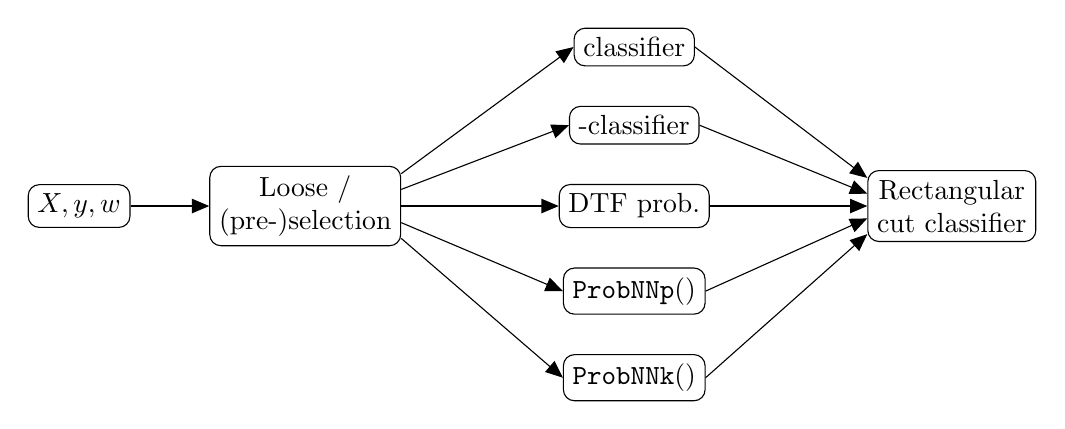
\begin{tikzpicture}[>=triangle 45,
                        node/.style={rectangle,align=center,rounded corners}]
        \node[draw,node] (data) {$X, y, w$};
        \node[draw,node,right=1cm of data] (presel) {Loose / \\ (pre-)selection};
        \node[draw,node,right=2cm of presel] (dtf) {DTF prob.};
        \node[draw,node,above=.5cm of dtf] (clfLbDz) {\Lb-\Dz classifier};
        \node[draw,node,above=.5cm of clfLbDz] (clfLz) {\Lz classifier};
        \node[draw,node,below=.5cm of dtf] (pProbNNp) {\texttt{ProbNNp}$(\proton)$};
        \node[draw,node,below=.5cm of pProbNNp] (kProbNNk) {\texttt{ProbNNk}$(\kaon)$};
        \node[draw,node,right=2cm of dtf] (fclf) {Rectangular\\ cut classifier};

        \draw[->] (data) -- (presel);
        \draw[->] (presel) -- (dtf);
        \draw[->] (presel.north east) + (0,-1mm) -- (clfLz.west);
        \draw[->] (presel.north east) + (0,-3mm) -- (clfLbDz.west);
        \draw[->] (presel.south east) + (0, 3mm) -- (pProbNNp.west);
        \draw[->] (presel.south east) + (0, 1mm) -- (kProbNNk.west);
        \draw[->] (dtf) -- (fclf);
        \draw[->] (clfLz.east) -- ($(fclf.north west) + (0,-1mm)$);
        \draw[->] (clfLbDz.east) -- ($(fclf.north west) + (0,-3mm)$);
        \draw[->] (pProbNNp.east) -- ($(fclf.south west) + (0,3mm)$);
        \draw[->] (kProbNNk.east) -- ($(fclf.south west) + (0,1mm)$);
    \end{tikzpicture}
    \caption{Data flow of the \gls{mva}. The data matrix $X \in \mathbb{R}^{m \times n}$ ($m$ instances and $n$ features), respective labels $y \in \mathbb{R}^m$ and weights $w \in \mathbb{R}^m$ are filtered by the preselection and loose selection step and then pass through two tiers of \glspl{mva}.}
    \label{fig:LbToDzLz_mvaoutline}
\end{figure}
The reason behind the outlined design decision, as well as detailed explanations of the classifiers are given in the following sections and in Appx.~\ref{chap:apdx_mva_xcheck}.

\subsection{The Data Pipeline}
\label{sec:mvaLz_datapipeline}
Before the data are fed into the different \gls{mva} algorithms, certain transformation and filtering steps have to be applied.
Most steps are necessary for the training and evaluation step (\eg{}, standardization), whereas others (\eg{}, balancing) should only be applied during training.
Formally, we split the training and evaluation phase into the two separate steps \textit{fit} and \textit{transform} and implement them as steps of a pipeline as shown in Fig.~\ref{fig:mvaLz_filter_transform}.
During the \textit{fit} step only certain rows (\ie{}, instances) of $X$, $y$ and $w$ are selected which reflects balancing and cross-validation.
(The technique of cross-validation as used in the present analysis in explained in Appx.~\ref{chap:crossval}.)
Features that are used for the training of one of the classifiers are 
\begin{enumerate}[itemsep=2pt,parsep=2pt]
    \item standardized,
    \item decorrelated according to the respective signal distributions via a \gls{pca} transformation, and
    \item subsequently ordered w.r.t.\ the Wasserstein distance (signal vs.\ background) of the respective \gls{pca} components,
\end{enumerate}
where the last two steps are skipped for \glspl{svm}.
Each of these steps involves a trivial fitting step (\eg{}, finding the mean and standard deviation for the standardization) which then yields parameters that are used to transform the data.
These parameters are obtained during the training step (\textit{fit} pipeline) and are kept constant during the evaluation step.
Fixing these values during the latter step is important, since, for instance, the mean of a given feature can deviate between the training and testing sample (\ie{}, $(X,y,w) \neq (X',y',w')$ in Fig.~\ref{fig:mvaLz_filter_transform}).
\begin{sidewaysfigure}[htbp]
    \centering
    \begin{subfigure}{\textwidth}
        \centering
        \includegraphics[scale=1.]{mvaLz/fit.png}
        \caption{Fit}
    \end{subfigure}
    \par\bigskip 
    \begin{subfigure}{\textwidth}
        \centering
        \includegraphics[scale=1.]{mvaLz/transform.png}
        \caption{Transform}
    \end{subfigure}
    \caption{Fit and transform step as described in Sec.~\ref{sec:mvaLz_datapipeline}. The former fits parameters of various transform steps (\eg{}, \textit{Transform \#1}) which are fixed during evaluation of the latter.}
    \label{fig:mvaLz_filter_transform}
\end{sidewaysfigure}

The standardization of features helps to improve the performance of classifiers that are sensitive to the (different) scales of the features (\eg{}, \glspl{svm}), whereas the decorrelation step increases the performance of classifiers that are based on rectangular selection requirements (\eg{}, decision trees).
We note that the evaluation of the mean and standard deviation, as well as the correlation matrix is carried out on a balanced subset of the available data (\textit{fit} pipeline) and will therefore not necessarily standardize or decorrelate the entire data set.
The ordering of the \gls{pca} components allows a first order approximation of the importance hierarchy of the features.
The decorrelation via \gls{pca} transformation, as well as the subsequent ordering via the Wasserstein metric is elaborated in Appx.~\ref{chap:pca}.

\subsection{The \texorpdfstring{\Lz}{Λ} Classifier}
\label{sec:LbToDzLz_mvaLz}
The \Lz classifier is designed to increase the purity of the \Lz candidates, \ie{}, the trained classifier should have learned to identify genuine \decay{\Lz}{\proton\pim} decays and reject random combinations, as well as \glspl{reflection}.
It is therefore trained on the lower and upper sidebands of the invariant mass distribution $m(\proton\pim)$ (background) and with calibrated \gls{truthmatched} \gls{mc} simulated events (signal).

The detector response critically depends on the lifetime of the \Lz baryon (\ie{}, the track type of the \Lz daughters) as discussed previously.
We therefore split the samples w.r.t.\ to the track types \gls{LL} and \gls{DD} and train two separate classifiers.
The invariant mass distribution $m(\proton\pim)$ as well as the sideband boundaries are shown in Fig.~\ref{fig:mvaLz_hLzM}.
The numerical values for the sideband boundaries are listed in Tab.~\ref{tab:mvaLz_defsidebands}.
\begin{figure}[htbp]
    \centering
    \begin{subfigure}[b]{.49\textwidth}
        \centering
        \includegraphics[scale=1.]{mvaLz/hLzM_LL.png}
    \end{subfigure}
    \begin{subfigure}[b]{.49\textwidth}
        \centering
        \includegraphics[scale=1.]{mvaLz/hLzM_DD.png}
    \end{subfigure}
    \caption{Distribution of the invariant mass of \Lz candidates after the loose selection for the different track types \gls{LL} (left) and \gls{DD} (right). The dashed lines indicate the sidebands used for training the \Lz classifier.}
    \label{fig:mvaLz_hLzM}
\end{figure}

\begin{table}[htbp]
    \centering
    \caption{Definition of the low and high edge of the lower and upper sidebands of $m(\proton\pim)$. The different sizes for \gls{LL} and \gls{DD} tracks are motivated by the different signal peak resolution and the amount of available data.}
    \label{tab:mvaLz_defsidebands}
    \begin{tabular}{lSSSS}
        \toprule
        & \multicolumn{2}{c}{{lower sideband}} & \multicolumn{2}{c}{{upper sideband}} \\
        & {low [\gevcc]} & {high [\gevcc]} & {low [\gevcc]} & {high [\gevcc]} \\
        \midrule
        \gls{LL} & 1.090 & 1.107 & 1.125 & 1.140 \\
        \gls{DD} & 1.090 & 1.104 & 1.128 & 1.140 \\
        \bottomrule
    \end{tabular}
\end{table}

In order to find the efficiency of the final classifier, we split the data sample into a training and a test sample.
Subsequently, the classifier is optimized and trained on the former and eventually evaluated on the latter.
The ratio of the sizes of the training and test samples is the objective of a min-max problem:
A large training sample allows low-biased, complex classifier but the evaluation of the efficiency on the testing sample also comes with a large uncertainty due to the low statistics of this sample. 
Let $p$ be the true signal efficiency of the classifier that categorizes $n_\text{sig}$ signal and $n_\text{bkg}$ background events from $n = n_\text{sig} + n_\text{bkg}$ given instances:
\begin{equation*}
    p := \frac{n_\text{sig}}{n} \,.
\end{equation*}
Its uncertainty $u_p$ is then given by the standard deviation of a binomial distribution
\begin{equation*}
    \frac{u_p}{p} = \sqrt{\frac{1 - p}{p} \, \frac{1}{n}} \,.
\end{equation*}
For estimation, $n$ is the number of (\gls{mc} simulated) signal events in the testing sample and $n_\text{sig}$ ($n_\text{bkg})$ is the number of \gls{tp} (\gls{fn}).
In Fig.~\ref{fig:mvaLz_uefficiency_theory} we show the amount of (\gls{mc} simulated) signal events that corresponds to $1\,\%$, $5\,\%$ and $10\,\%$ uncertainty of the classifier efficiency as a function of the efficiency itself.
We choose $n=1000$ which corresponds to a sub $5\,\%$ uncertainty for classifier efficiencies above $30\,\%$.
\begin{figure}[htbp]
    \centering
    \includegraphics[scale=1.]{mvaLz/uefficiency_theory.png}
    \caption{Amount of events $n$ that corresponds to $1\,\%$, $5\,\%$ and $10\,\%$ uncertainty of the classifier efficiency as a function of the efficiency itself.}
    \label{fig:mvaLz_uefficiency_theory}
\end{figure}

It is well known that imbalanced data in classification tasks can reduce classification power of classifiers dramatically by having a bias towards the majority classes in the data set~\cite{imbalclf1,imbalclf2}.
We therefore balance our dataset each time before training one of our classifiers and since the accuracy is limited by the amount of available (\gls{mc} simulated) signal events anyhow, we also prune our dataset with \gls{DD} tracks for the evaluation steps for the sake of computational ease.
In Tab.~\ref{tab:mvaLz_ndata} we list the sizes of the pruned trainings and testing sets for \gls{LL} and \gls{DD} tracks.
An additional pruning to balance the data set, as described in Sec.~\ref{sec:mvaLz_datapipeline}, happens during the training step and is not reflected in Tab.~\ref{tab:mvaLz_ndata}.

\begin{table}[htbp]
    \centering
    \caption{Sizes of training and testing samples for \gls{LL} and \gls{DD} tracks used for the \gls{mva}. (The background sample (rec.\ data) was pruned in a previous step.)}
    \label{tab:mvaLz_ndata}
    \begin{tabular}{l
                    S[table-format=5.0]
                    S[table-format=5.0]
                    S[table-format=5.0]
                    S[table-format=5.0]}
        \toprule
        & \multicolumn{2}{c}{{\gls{LL}}} & \multicolumn{2}{c}{{\gls{DD}}} \\
        {Label} & {Training} & {Testing} & {Training} & {Testing} \\
        \midrule
        Signal & 10491 & 1000 & 26176 & 1000 \\
        %Background & 8951 & 10000 & 50000 & 10000 \\
        Background & 10151 & 10000 & 50000 & 10000 \\
        \bottomrule
    \end{tabular}
\end{table}

We train five classifiers (twice for \gls{LL} and \gls{DD} tracks) using different machine learning algorithms for each (tier~1.1), as well as a stacking classifier (tier~1.2), which combines the output of the former five classifiers.
In Tab.~\ref{tab:mvaLzLbDz_hyperparams} we list the classifiers, as well as their respective hyper-parameters and whether or not they were optimized or fixed during the training phase.
\begin{table}[htbp]
    \centering
    \caption{Hyper-parameters of the \Lz classifiers and \Lb-\Dz classifiers. Parameter values are optimized via a 5-fold cross-validation if not marked with $\dagger$.}
    \label{tab:mvaLzLbDz_hyperparams}
    \begin{tabular}{lllll}
        \toprule
        && \multicolumn{2}{c}{Value} \\
        Classifier & Hyper-parameter & \Lz Clf. & \Lb-\Dz Clf. \\
        \midrule
        \midrule
        \Gls{svm} & Kernel & RBF${}^\dagger$ & RBF${}^\dagger$ \\
        & $\gamma$ (kernel coefficient) & $0.1$ & $0.1$ \\
        & $C$ (regularization) & $50$ (\gls{LL}), $1$ (\gls{DD}) & $1$ (\gls{LL}), $5$ (\gls{DD}) \\
        \midrule
        Extra Trees & Criterion & Gini${}^\dagger$ & Gini${}^\dagger$ \\
        & Number of trees & $100$ & $100$ \\
        & Max.\ depth & $10$ & $20$ \\
        \midrule
        Random Forest & Criterion & Gini${}^\dagger$ & Gini${}^\dagger$ \\
        & Number of trees & $100$ & $100$ \\
        & Max.\ depth & $10$ & $20$ \\
        \midrule
        \Gls{bdt} & Loss & Deviance${}^\dagger$ & Deviance${}^\dagger$ \\
        & Criterion & Friedman MSE${}^\dagger$ & Friedman MSE${}^\dagger$ \\
        & Number of trees & $100$ & $100$ \\
        & Max.\ depth & $5$ & $5$ \\
        \midrule
        Ada.\ \gls{bdt} & Loss & Exponential${}^\dagger$ & Exponential${}^\dagger$ \\
        & Criterion & Friedman MSE${}^\dagger$ & Friedman MSE${}^\dagger$ \\
        & Number of trees & $100$ & $100$ \\
        & Max.\ depth & $5$ & $5$ \\
        \midrule
        Stacking & Kernel & RBF${}^\dagger$ & -- \\
        & $\gamma$ (kernel coefficient) & $0.1$ &  -- \\
        & $C$ (regularization) & $10$ & -- \\
        \bottomrule
    \end{tabular}
\end{table}

\subsubsection{Tier~1.1}
The five tier~1.1 classifiers are
\begin{enumerate}[itemsep=2pt,parsep=2pt]
    \item a \gls{svm},
    \item Extra Trees,
    \item a Random Forest,
    \item a \gls{bdt} using gradient boosting, and
    \item a \gls{bdt} using adaptive boosting.
\end{enumerate}
We give a short introduction, as well as an explanation of the hyper-parameters listed in Tab.~\ref{tab:mvaLzLbDz_hyperparams} for \glspl{svm} in Appx.~\ref{chap:svm}, as well as for the ensemble learning algorithms (2.\ - 5.) in Appx.~\ref{chap:apdx_forest}.
The hyper-parameters are optimized in a 5-fold cross-validation scheme (\cf{}~Appx.~\ref{chap:crossval}) where the optimization objective is the \gls{rocauc} in the aggregation of the testing folds (\ie{}, not the previously separated testing set).
In Fig.~\ref{fig:mvaLz_svm_hyperparams}, Fig.~\ref{fig:mvaLz_forest_hyperparams} and Fig.~\ref{fig:mvaLz_bdt_hyperparams} we show the \gls{rocauc} on the testing and the training folds for different hyper-parameter configurations.
Plotting the latter has the advantage to easily identify configurations that suffer from overfitting (large difference between \gls{rocauc} values), and low variance but high bias configurations (small \gls{rocauc} values).
The desired maximum is typically located at the point in configuration space where the \gls{rocauc} values between testing and training folds start to diverge.
The evaluation of the \glspl{svm} are computationally intense (\cf{}~Appx.~\ref{chap:svm}).
We therefore only scan two slices of the two-dimensional $C$-$\gamma$ configuration space, whereas we use full grid-search for optimizing the decision tree ensembles.
The points $(C,\gamma)=(50,0.1)$ and $(C,\gamma)=(1,0.1)$ for \gls{LL} and \gls{DD} tracks, respectively, are scanned twice by the former technique and yield slightly different \gls{rocauc} values due to the randomized partitioning.\footnote{The estimation of the performance of the final classifier is not obtained via cross-validation but on the separated testing set. Hence, no uncertainty due to fluctuation in the cross-validation processes is taken into account for subsequent steps.}

Ever since the advent of neural networks, early stopping (\eg{}, Ref.~\cite{earlystopping_gd}) has become a commonly used regularization technique approach to prevent models to perform badly in the testing set after training a certain amount of iterations\footnote{In the context of neural networks another commonly used technique is \textit{Dropout}.} (\eg{}, Ref.~\cite{earlystopping_nn}).
The very same behavior due to overfitting is observed when using boosting techniques in particular, or gradient descent techniques in general, and early stopping techniques have proven to be an effective antidote \cite{earlystopping_boosting1,earlystopping_boosting2}.
Whereas additional regularization is required for these kind of learners, a key advantage of \glspl{svm} is their intrinsic regularization such that additional regularization by applying early stopping is not necessary here, albeit occasionally applied in order to shortcut training time~\cite{earlystopping_svm}.
We therefore use early stopping techniques for training the ensemble learners (at each point in the hyper-parameter configuration space) to prevent overfitting and rely on intrinsic regularization of \glspl{svm}.
A consistency check for the latter assumption is given by the convergence behavior of the \glspl{svm} shown in Fig.~\ref{fig:mvaLz_convergence}.

\begin{figure}[htbp]
    \centering
    \begin{subfigure}[b]{.49\textwidth}
        \centering
        \includegraphics[scale=1.]{mvaLz/svm_C_LL.png}
    \end{subfigure}
    \begin{subfigure}[b]{.49\textwidth}
        \centering
        \includegraphics[scale=1.]{mvaLz/svm_C_DD.png}
    \end{subfigure}
    \par\bigskip 
    \begin{subfigure}[b]{.49\textwidth}
        \centering
        \includegraphics[scale=1.]{mvaLz/svm_gamma_LL.png}
    \end{subfigure}
    \begin{subfigure}[b]{.49\textwidth}
        \centering
        \includegraphics[scale=1.]{mvaLz/svm_gamma_DD.png}
    \end{subfigure}
    \caption{Performance of the \gls{svm} (\Lz classifier) measured with the \gls{rocauc} for different values of the hyper-parameter $C$ (top) and $\gamma$ (bottom) and track types \gls{LL} (left) and \gls{DD} (right). The performance is evaluated via a 5-fold cross-validation which explains the minor fluctuation of configurations that are evaluated twice.}
    \label{fig:mvaLz_svm_hyperparams}
\end{figure}

\begin{figure}[htbp]
    \centering
    \begin{subfigure}[b]{.49\textwidth}
        \centering
        \includegraphics[scale=1.]{mvaLz/etrees_ntrees_LL.png}
        \caption{Extra Trees (\gls{LL})}
    \end{subfigure}
    \begin{subfigure}[b]{.49\textwidth}
        \centering
        \includegraphics[scale=1.]{mvaLz/etrees_ntrees_DD.png}
        \caption{Extra Trees (\gls{DD})}
    \end{subfigure}
    \par\bigskip 
    \begin{subfigure}[b]{.49\textwidth}
        \centering
        \includegraphics[scale=1.]{mvaLz/rforest_ntrees_LL.png}
        \caption{Random Forest (\gls{LL})}
    \end{subfigure}
    \begin{subfigure}[b]{.49\textwidth}
        \centering
        \includegraphics[scale=1.]{mvaLz/rforest_ntrees_DD.png}
        \caption{Random Forest (\gls{DD})}
    \end{subfigure}
    \caption{Performance of Extra Trees (top) and a Random Forest (bottom) measured with the \gls{rocauc} for different values for the maximal allowed tree depth~($x$-axis) and number of trees~($n$), evaluated on the testing folds~(solid lines) and training folds~(dashed lines).}
    \label{fig:mvaLz_forest_hyperparams}
\end{figure}

\begin{figure}[htbp]
    \centering
    \begin{subfigure}[b]{.49\textwidth}
        \centering
        \includegraphics[scale=1.]{mvaLz/gboosting_ntrees_LL.png}
        \caption{Gradient boosting (\gls{LL})}
    \end{subfigure}
    \begin{subfigure}[b]{.49\textwidth}
        \centering
        \includegraphics[scale=1.]{mvaLz/gboosting_ntrees_DD.png}
        \caption{Gradient boosting (\gls{DD})}
    \end{subfigure}
    \par\bigskip 
    \begin{subfigure}[b]{.49\textwidth}
        \centering
        \includegraphics[scale=1.]{mvaLz/aboosting_ntrees_LL.png}
        \caption{Adaptive boosting (\gls{LL})}
    \end{subfigure}
    \begin{subfigure}[b]{.49\textwidth}
        \centering
        \includegraphics[scale=1.]{mvaLz/aboosting_ntrees_DD.png}
        \caption{Adaptive boosting (\gls{DD})}
    \end{subfigure}
    \caption{Performance of \gls{bdt} classifiers (using gradient (top) and adaptive (bottom) boosting) measured with the \gls{rocauc} for different values for the maximal allowed tree depth~($x$-axis) and number of trees~($n$), evaluated on the testing folds~(solid lines) and training folds~(dashed lines).}
    \label{fig:mvaLz_bdt_hyperparams}
\end{figure}

\begin{figure}[htbp]
    \centering
    \begin{subfigure}[b]{.49\textwidth}
        \centering
        \includegraphics[scale=1.]{mvaLz/convergence_LL.png}
        \caption{\gls{LL} tracks}
    \end{subfigure}
    \begin{subfigure}[b]{.49\textwidth}
        \centering
        \includegraphics[scale=1.]{mvaLz/convergence_DD.png}
        \caption{\gls{DD} tracks}
    \end{subfigure}
    \caption{Convergence of the \glspl{svm} (\Lz classifier) given by the \gls{rocauc} values for different sample sizes where a sample size of $100\,\%$ corresponds to the size of the full trainings set. The \gls{rocauc} is evaluated via a 5-fold cross-validation scheme on the training (solid line) and testing folds (dashed line).}
    \label{fig:mvaLz_convergence}
\end{figure}

\subsubsection{Tier 1.2 (Stacking)}
In the second tier we aggregate the output of the classifiers of tier~1.1 and use them as the feature set of a next classifier.
Again, the features are transformed before the training phase of the tier~1.2 classifier begins.
The transformation involves a standardization and subsequent decorrelation via a \gls{pca} transformation, followed by a sorting of the \gls{pca} components w.r.t.\ their separation power between signal and background, measured in the Wasserstein $l_1$ metric.
The feature set before and after decorrelation is shown in Fig.~\ref{fig:mvaLz_stack_features_LL}, Fig.~\ref{fig:mvaLz_stack_features_DD}, and Fig.~\ref{fig:mvaLz_stack_pcafeatures_LL}, Fig.~\ref{fig:mvaLz_stack_pcafeatures_DD}, respectively.
A strong correlation among the features is apparent, pointing towards a redundancy of the classifiers due to an exhaustion of the available information which resembles the findings of Refs.~\cite{unreasonableeffdata1,unreasonableeffdata2}.
We account for this degeneration by only using the first and second \gls{pca} components in the tier~1.2 classifier.
We use a \gls{svm} with an RBF kernel for classifying the two-dimensional feature set and optimize the corresponding hyper-parameters $C$ and $\gamma$ via a 5-fold cross-validation scheme.
The results are listed in Tab.~\ref{tab:mvaLzLbDz_hyperparams} (referred to as \textit{Stacking}) and shown visually in Fig.~\ref{fig:mvaLz_stack_hyperparams}.
Additionally, the limited size of the feature set allows for a simple graphical representation of the decision boundary of the optimized classifier which is given in Fig.~\ref{fig:mvaLz_decboundary}.

\begin{figure}[htbp]
    \centering
    \begin{subfigure}[b]{.49\textwidth}
        \centering
        \includegraphics[scale=1.]{mvaLz/stack_C_LL.png}
    \end{subfigure}
    \begin{subfigure}[b]{.49\textwidth}
        \centering
        \includegraphics[scale=1.]{mvaLz/stack_C_DD.png}
    \end{subfigure}
    \par\bigskip 
    \begin{subfigure}[b]{.49\textwidth}
        \centering
        \includegraphics[scale=1.]{mvaLz/stack_gamma_LL.png}
    \end{subfigure}
    \begin{subfigure}[b]{.49\textwidth}
        \centering
        \includegraphics[scale=1.]{mvaLz/stack_gamma_DD.png}
    \end{subfigure}
    \caption{Performance of the stacking classifier (\gls{svm} with an RBF kernel) measured with the \gls{rocauc} for different values of the hyper-parameter $C$ and $\gamma$, evaluated via a 5-fold cross-validation scheme.}
    \label{fig:mvaLz_stack_hyperparams}
\end{figure}

\begin{figure}[htbp]
    \centering
    \begin{subfigure}[b]{.49\textwidth}
        \centering
        \includegraphics[scale=1.]{mvaLz/stack_corr_LL.png}
    \end{subfigure}
    \begin{subfigure}[b]{.49\textwidth}
        \centering
        \includegraphics[scale=1.]{mvaLz/stack_corr_DD.png}
    \end{subfigure}
    \caption{Decision boundary for \gls{LL} (left) and \gls{DD} (right) tracks of the stacking classifier (\gls{svm} with an RBF kernel) overlayed with 400 instances of the signal and background class (200 each). The signal (background) class is depicted with circles (triangles) and the corresponding classifier response in blue (red).}
    \label{fig:mvaLz_decboundary}
\end{figure}

\subsubsection{Evaluation}
The performance of all trained classifiers are judged w.r.t.\ their \gls{rocauc} values, evaluated on the separated testing set.
The corresponding \gls{roc} curves are shown in Fig.~\ref{fig:mvaLz_rocs} for \gls{LL} and \gls{DD} tracks.
\begin{figure}[htbp]
    \centering
    \includegraphics[scale=1.]{mvaLz/rocs.png}
    \caption{\Gls{roc} curves of the optimized \Lz classifiers, evaluated on the testing set.}
    \label{fig:mvaLz_rocs}
\end{figure}
\begin{table}[htbp]
    \centering
    \caption{\Gls{rocauc} values in percent for tier~1.1 and tier~1.2 \Lz classifiers (separately trained for \gls{LL} and \gls{DD} tracks), evaluated on the training and testing set.}
    \begin{tabular}{lSSSS}
        \toprule
        & \multicolumn{2}{c}{{Training}} & \multicolumn{2}{c}{{Testing}} \\
        Classifier & {\gls{LL} [\%]} & {\gls{DD} [\%]} & {\gls{LL} [\%]} & {\gls{DD} [\%]} \\
        \midrule
        \Gls{svm} & 93.25 & 82.92 & 92.86 & 83.25 \\
        Extra Tree & 93.02 & 82.69 & 91.45 & 82.44 \\
        Random Forest & 96.50 & 87.07 & 92.34 & 83.38 \\
        \Gls{bdt} & 95.30 & 85.16 & 92.60 & 83.47 \\ 
        Ada. \gls{bdt} & 94.92 & 84.86 & 92.51 & 83.37 \\
        Stacking & 95.46 & 87.57 & 90.87 & 80.42 \\
        \bottomrule
    \end{tabular}
\end{table}
The training of the stacking classifier (tier~1.2) does not show any improvement over the tier~1.1 classifiers.
For the sake of consistency (also with the \Lb-\Dz classifier), we therefore use the tier~1 \gls{svm} as our final classifier, both for \gls{LL} and \gls{DD} tracks.
The response, as well as the efficiency for given thresholds are shown graphically in Fig.~\ref{fig:mvaLz_response}.
Further, we show the distribution of the marginal and linear correlation distributions of the five-dimensional feature space before and after the \gls{pca} transformation in Fig.~\ref{fig:mvaLz_corr_LL}, Fig.~\ref{fig:mvaLz_corr_DD} and Fig.~\ref{fig:mvaLz_pcacorr_LL}, Fig.~\ref{fig:mvaLz_pcacorr_DD}, where we color-coded misclassified events in red (signal events classified as background) and blue (background events classified as signal) when using a threshold of zero.
\begin{figure}[htbp]
    \centering
    \includegraphics[scale=1.]{mvaLz/response.png}
    \caption{Efficiency (solid and dashed line) when using a given threshold ($x$-axis) for classifying signal and background, and response function (histogram) of the tier~1 \gls{svm} (\Lz classifier), trained separately for \gls{LL} (left) and \gls{DD} (right) tracks.}
    \label{fig:mvaLz_response}
\end{figure}

\begin{figure}[htbp]
    \centering
    \includegraphics[scale=1.]{mvaLz/mvaLz_corr_LL.png}
    \caption{Marginal and linear correlation distributions of the feature space (\Lz classifier) before applying \gls{pca} transformation for \gls{LL} tracks. In the correlation distributions misclassified events are color-coded in red (signal events classified as background) and blue (background events classified as signal) when using a threshold of zero.}
    \label{fig:mvaLz_corr_LL}
\end{figure}

\begin{figure}[htbp]
    \centering
    \includegraphics[scale=1.]{mvaLz/mvaLz_corr_DD.png}
    \caption{Marginal and linear correlation distributions of the feature space (\Lz classifier) before applying \gls{pca} transformation for \gls{DD} tracks. In the correlation distributions misclassified events are color-coded in red (signal events classified as background) and blue (background events classified as signal) when using a threshold of zero.}
    \label{fig:mvaLz_corr_DD}
\end{figure}

\begin{figure}[htbp]
    \centering
    \includegraphics[scale=1.]{mvaLz/mvaLz_pcacorr_LL.png}
    \caption{Marginal and linear correlation distributions of the \gls{pca} components (\Lz classifier) for \gls{LL} tracks. In the correlation distributions misclassified events are color-coded in red (signal events classified as background) and blue (background events classified as signal) when using a threshold of zero.}
    \label{fig:mvaLz_pcacorr_LL}
\end{figure}

\begin{figure}[htbp]
    \centering
    \includegraphics[scale=1.]{mvaLz/mvaLz_pcacorr_DD.png}
    \caption{Marginal and linear correlation distributions of the \gls{pca} components (\Lz classifier) for \gls{DD} tracks. In the correlation distributions misclassified events are color-coded in red (signal events classified as background) and blue (background events classified as signal) when using a threshold of zero.}
    \label{fig:mvaLz_pcacorr_DD}
\end{figure}


\subsection{The \texorpdfstring{\Lb-\Dz}{Λb-D} Classifier}
\label{sec:LbToDzLz_mvaLbDz}
The \Lb-\Dz classifier is trained and optimized very similar to the \Lz classifier that we described in the previous section.
Differences are the increased feature set (10 features instead of 5) and the fact that the background sample for the \Lb-\Dz classifier is the full recorded \decay{\Lb}{\Dz\Lz} data set, rather than sidebands as used for training the \Lz classifier.
The decision for the latter is motivated by the fact that classification algorithms typically tolerate impure labels (\eg{}, Ref.~\cite{cwola,weaklysupclass}) and that the expected impurity in the case $m(\Dz\Lz)$ is extremely low.
At the same time, this approach minimizes the risk of a selection bias by a non-trivial correlation of the invariant mass $m(\Dz\Lz)$ and the feature set.
The invariant mass distribution $m(\Dz\Lz)$ is shown in Fig.~\ref{fig:mvaLbDz_hDzLzM} and is apparently dominated by combinatorial background.
Separation of the latter and genuine \decay{\Lb}{\Dz\Lz} decays is thus the main objective of the \Lb-\Dz classifier.

The approximation of the performance of the classifiers is limited by the amount of available \gls{mc} simulated events (signal) and, for the sake of computational ease, the data set is pruned, yielding the same sample sizes as listed in Tab.~\ref{tab:mvaLz_ndata}, except for a larger training set of \gls{LL} tracks (pruned to \num{20000} instances).
We test and optimize the same type of classifiers as we did in the previous section and thereby find, that the \gls{svm} performs best and that a stacking classifier does not help to improve the overall performance.
For the sake of brevity we thus suppress the separation into tier~1.1 and tier~1.2 and only list the results of tier~1.1 in the following.
The optimized hyper-parameter of the classifiers are listed in Tab.~\ref{tab:mvaLzLbDz_hyperparams}.

A key feature of a \gls{pca} analysis, especially when paired with ordering w.r.t.\ the separation power (as proposed in Appx.~\ref{chap:pca}) is the possibility to reduce the feature set and thus evade the \textit{curse of dimensionality}\footnote{In order to train learner effectively and avoid overfitting, the number of training instances should increase with the number of features. The \textit{Curse of dimensionality}~\cite{curseofdim} describes the highly non-linear relation between both which can lead to a reduced performance if the amount of the former is limited. A common mitigation is to reduce the number of features and only concentrate on the most important ones, \eg{}, via \gls{pca} transformation. Other and more complex dimensionality reduction schemes are Kernel PCA~\cite{kernelpca} or LLE~\cite{lle} (which both come with an additional set of hyper-parameters that have to be learned).} up to a certain degree.
In Fig.~\ref{fig:mvaLbDz_nfeatures} we show the \gls{rocauc} value (evaluated on the test set) for the different classifiers, when only the first $n=2$ to $10$ \gls{pca} components are used for the training.
Even though the beginning of saturation is visible after $n \gtrapprox 7$, the performance gain still justifies the increasing of the dimensionality of the feature space.
Hence, we use the full available feature set and use the \gls{pca} transformation to decorrelate the feature set (without reduction) in order to increase the performance of the decision tree based classifiers.

\begin{figure}[htbp]
    \centering
    \begin{subfigure}[b]{.49\textwidth}
        \centering
        \includegraphics[scale=1.]{mvaLbDz/nfeatures_LL.png}
    \end{subfigure}
    \begin{subfigure}[b]{.49\textwidth}
        \centering
        \includegraphics[scale=1.]{mvaLbDz/nfeatures_DD.png}
    \end{subfigure}
    \caption{\gls{rocauc} values (evaluated on the test set) for the different \Lb-\Dz classifiers, when only the first $n=2$ to $10$ \gls{pca} components (ordered w.r.t.\ the separation power) are used for the training.}
    \label{fig:mvaLbDz_nfeatures}
\end{figure}

The output, as well as the correlation of the classifiers are shown in Fig.~\ref{fig:mvaLbDz_stack_features_LL} and Fig.~\ref{fig:mvaLbDz_stack_features_DD}.
The corresponding \gls{rocauc} values are listed in Tab.~\ref{tab:mvaLbDz_rocaucs}.
By not only evaluating the \gls{rocauc} values on the testing set of corresponding track type, but also on the other set (as listed in Tab.~\ref{tab:mvaLbDz_rocaucs}), it is possible to verify the necessity of splitting the \Lb-\Dz classifiers w.r.t.\ the track type of \Lz (candidate) daughters.
An impact of the latter cannot be assumed a priori, but seemingly influences the performance of the classifiers (for instance via resolution dependent correlations) such that it makes sense (a posteriori) to split the available data set and train into two, rather than one, specialized classifiers.

\begin{figure}[htbp]
    \centering
    \includegraphics[scale=1.]{mvaLbDz/stack_features_LL_train.png}
    \caption{Distributions of the responses and correlations of the \Lb-\Dz classifiers for \gls{LL} tracks, separated for signal (S) and background (B). On top of the correlation distributions, we show the \gls{pcc} as a measure for the linear correlation.}
    \label{fig:mvaLbDz_stack_features_LL}
\end{figure}

\begin{figure}[htbp]
    \centering
    \includegraphics[scale=1.]{mvaLbDz/stack_features_DD_train.png}
    \caption{Distributions of the responses and correlations of the \Lb-\Dz classifiers for \gls{DD} tracks, separated for signal (S) and background (B). On top of the correlation distributions, we show the \gls{pcc} as a measure for the linear correlation.}
    \label{fig:mvaLbDz_stack_features_DD}
\end{figure}

\begin{table}[htbp]
    \centering
    \caption{\Gls{rocauc} values in percent for tier~1.1 and tier~1.2 \Lb-\Dz classifiers (separately trained for \gls{LL} and \gls{DD} tracks). \gls{rocauc} values are evaluated on the testing sets of both track types, \eg{}, \textit{\gls{LL} trained} and \textit{\gls{DD} tested} refers to the \gls{rocauc} value of a classifier that was trained with \gls{LL} tracks, but evaluated on the testing set with \gls{DD} track candidates.}
    \label{tab:mvaLbDz_rocaucs}
    \begin{tabular}{lSSSSSSSS}
        \toprule
        & \multicolumn{2}{c}{{\gls{LL} trained}} & \multicolumn{2}{c}{{\gls{DD} trained}} \\
        Classifier & {\gls{LL} tested [\%]} & {\gls{DD} tested [\%]} & {\gls{LL} tested [\%]} & {\gls{DD} tested [\%]} \\
        \midrule
        \Gls{svm} & 91.09 & 89.34 & 83.71 & 94.51 \\
        Extra Tree & 90.87 & 79.05 & 84.16 & 94.00 \\
        Random Forest & 90.68 & 82.29 & 83.15 & 94.17 \\
        \Gls{bdt} & 91.33 & 82.93 & 84.19 & 94.44 \\
        Ada. \gls{bdt} & 91.33 & 82.93 & 84.19 & 94.44 \\
        Stacking & 91.32 & 82.25 & 84.12 & 94.43 \\
        \bottomrule
    \end{tabular}
\end{table}

Resting on the \gls{rocauc} values of the classifiers, we again chose the \gls{svm} as the \Lb-\Dz classifier.
The respective \gls{roc} curves for \gls{LL} and \gls{DD} tracks, as well as the response functions are shown in Fig.~\ref{fig:mvaLzLbDz_roc} and Fig.~\ref{fig:mvaLbDz_response}, respectively.
Similar to Sec.~\ref{sec:LbToDzLz_mvaLz}, we investigate the convergence of the \gls{svm} and show the result in Fig.~\ref{fig:mvaLbDz_convergence}.

\begin{figure}[htbp]
    \centering
    \includegraphics[scale=1.]{mvaLbDz/response.png}
    \caption{Efficiency (solid and dashed line) when using a given threshold ($x$-axis) for classifying signal and background, and response function (histogram) of the \gls{svm} (\Lb-\Dz classifier), trained separately for \gls{LL} (left) and \gls{DD} (right) tracks.}
    \label{fig:mvaLbDz_response}
\end{figure}

\subsection{The Tier 2 Classifier}
After having trained optimized \Lz and \Lb-\Dz classifiers, we fuse the normalized output of these classifiers with the \gls{dtf} probability, as well as the output of \gls{pid} providing neural networks $\texttt{ProbNNp}(\proton)$ and $\texttt{ProbNNk}(\kaon)$, and use these five variables as the feature set of the Tier~2 classifier.
The (marginal) distribution, as well as the correlations of the feature set are shown in Fig.~\ref{fig:mva_features_LL} (\gls{LL} tracks) and Fig.~\ref{fig:mva_features_DD} (\gls{DD} tracks).
\begin{figure}[htbp]
    \centering
    \includegraphics[scale=1.]{mva/features_LL.png}
    \caption{Marginal distributions and correlations of the feature set of the Tier~2 classifier for \gls{LL} tracks. Instances of the \textit{signal} (S) and the \textit{background} (B) class are color-coded in blue and red, respectively.}
    \label{fig:mva_features_LL}
\end{figure}

\begin{figure}[htbp]
    \centering
    \includegraphics[scale=1.]{mva/features_DD.png}
    \caption{Marginal distributions and correlations of the feature set of the Tier~2 classifier for \gls{DD} tracks. Instances of the \textit{signal} (S) and the \textit{background} (B) class are color-coded in blue and red, respectively.}
    \label{fig:mva_features_DD}
\end{figure}

The Tier~2 classifier is intentionally kept rudimentary and applies only a single threshold requirement (rectangular cut) to each feature.
By design, each feature is expected to have values close to one for signal-like events, and values close to zero else.
The threshold requirement therefore reads as a required lower bound $t_i$ for each feature $f_i$, \ie{},
\begin{equation*}
    \text{signal} \; :\Leftrightarrow \; (f_1 > t_1) \; \land \; (f_2 > t_2) \; \land \; \ldots \; \land (f_5 > t_5) \,.
\end{equation*}
Doing so makes the Tier~2 classifier unable to learn any higher level features beyond the marginal distributions (such as correlation) of the features.
In particular this renders the need to recalibrate the \texttt{ProbNNp} and \texttt{ProbNNk} correlations in \gls{mc} simulated events unnecessary which is an error prone business and requires decent statistics.
In Appx.~\ref{chap:apdx_mva_xcheck} we find that selection requirements for the last three features introduce deviations between recorded and simulated data for thresholds close to one, whereas the fidelity of the first two features (\Lz and \Lb-\Dz classifier) is sufficient.
We will therefore not aggressively optimize thresholds requirements with the Tier~2 classifier, but choose loose selection requirements and tighten them in a subsequent step using only the output of the \Lz and \Lb-\Dz classifiers.

As a cross-check we compare the results with the decisions of a canonically trained binary decision tree (Gini criterion and max.\ depth of 5).
The \glspl{roc} of all classifiers (\ie{}, feature set and both Tier~2 variants) are shown in Fig.~\ref{fig:mva_rocs} and the respective \gls{rocauc} values are listed in Tab.~\ref{tab:mva_rocaucs}.

\begin{figure}[htbp]
    \centering
    \includegraphics[scale=1.]{mva/rocs.png}
    \caption{\Gls{roc} curves of the feature set used to train Tier~2, \ie{}, the decision tree (Dec.~Tree) and the rectangular cut classifier (Rec.\ Clf.), as well the respective \gls{roc} curves of the Tier~2 classifiers themselves. Note that we evaluated the rectangular classifier only for \gls{tpr} $< 90\,\%$ due to numerical instability.}
    \label{fig:mva_rocs}
\end{figure}

\begin{table}[htbp]
    \centering
    \caption{\Gls{rocauc} values in percent for Tier~2 \Lz classifiers (separately trained for \gls{LL} and \gls{DD} tracks), evaluated on the training and testing set. For numerical reasons, the \gls{roc} curve of the rectangular cut classifier (Rec.\ Clf.) is only evaluated for \gls{tpr} $< 90\,\%$ (\cf{}~Fig.~\ref{fig:mva_rocs}) which explains the inhibited \gls{rocauc} values for this classifier.}
    \label{tab:mva_rocaucs}
    \begin{tabular}{lSSSS}
        \toprule
        & \multicolumn{2}{c}{{Training}} & \multicolumn{2}{c}{{Testing}} \\
        Classifier & {\gls{LL} [\%]} & {\gls{DD} [\%]} & {\gls{LL} [\%]} & {\gls{DD} [\%]} \\
        \midrule
        \Lz Clf. & 93.46 & 82.93 & 89.48 & 82.09 \\
        \Lb-\Dz Clf. & 92.69 & 94.90 & 90.76 & 94.62 \\
        \Gls{dtf} prob. & 94.32 & 91.60 & 93.72 & 91.86 \\
        \texttt{ProbNN}(\proton) & 79.82 & 74.95 & 78.72 & 74.31 \\
        \texttt{ProbNN}(\kaon) & 86.32 & 84.82 & 85.96 & 84.61 \\
        \midrule
        Decision Tree & 97.74 & 96.96 & 96.77 & 96.78 \\
        Rec.\ Clf. & 94.98 & 93.67 & 94.86 & 93.06 \\
        \bottomrule
    \end{tabular}
\end{table}

\subsubsection{The Rectangular Cut Classifier}
For uncorrelated features, the relations between \gls{tpr}, \gls{fpr}, \gls{fnr} and \gls{tnr} (\cf{}~Appx.~\ref{chap:confmat} for our definitions of \textit{true}, \textit{false}, \textit{positive} and \textit{negative}) in the presence of rectangular selection requirements read
\begin{align*}
    \text{TPR} &= \text{TPR}_1 \times \text{TPR}_2 \times \ldots \,, \\
    \text{FPR} &= \text{FPR}_1 \times \text{FPR}_2 \times \ldots \,, \\
    \text{FNR} &= 1 - \text{TPR} = 1 - \text{FNR}_1 \times \text{FNR}_2 \times \ldots \,, \\
    \text{TNR} &= 1 - \text{FPR} = 1 - (1 - \text{TNR}_1) \times (1 - \text{TNR}_2) \times \ldots \,,
\end{align*}
and in particular $\text{TNR} \neq \prod_i \text{TNR}_i$.
In our case we are striving to minimize the overall \gls{fpr} for a given target \gls{tpr} $\hat p_\text{TPR}$ by requiring thresholds $\vec t$:
\begin{equation}
    \label{eq:recopt}
    \vec \nabla_{\vec t, \lambda} \mathcal{L} \overset{!}{=} 0 \quad \text{with} \quad \mathcal{L}\!\left(\vec{t}, \lambda \right) = \text{FPR}\!\left(\vec{t} \, \right) - \lambda \left[ \text{TPR}\!\left(\vec{t} \, \right) - \hat p_\text{TPR} \right] \,.
\end{equation}
In case of uncorrelated features
\begin{equation}
    \label{eq:recopt_init}
    \text{TPR}_i = (\hat p_\text{TPR})^{1/n}
\end{equation}
solves this optimization problem.
However, a certain degree of correlation is expected for the feature set of the Tier~2 classifier and we therefore have to solve Eq.~\eqref{eq:recopt} numerically.
The Lagrange multiplier $\lambda$ in Eq.~\eqref{eq:recopt} is unbound which makes numerical approaches difficult. Hence, we rewrite the problem as
\begin{equation}
    \label{eq:mva_siman}
    \vec \nabla_{\vec{t}} \, \mathcal{L} \overset{!}{=} 0 \quad \text{with} \quad \mathcal{L}\!\left(\vec{t} \, \right) = \text{FPR}\!\left(\vec{t} \, \right) + \underbrace{\log\!\left( \left| \text{TPR}\!\left(\vec{t} \, \right) - \hat p_\text{TPR} \right| + \epsilon \right)}_{\text{penalty}} \,.
\end{equation}
where we replaced the latter part of the Lagrangian function with a penalty term.
Due to the discontinuities of the derivatives of $\mathcal{L}$, gradient descent techniques will not work sufficiently.
We therefore use simulated annealing~\cite{simannealing} with initial values taken from Eq.~\eqref{eq:recopt_init} to find thresholds $\vec t$ for a given \gls{tpr} $\hat p_\text{TPR}$ while keeping the overall \gls{fpr} minimal.
This method becomes numerically unstable for $\hat p_\text{TPR}<0.1$ and $\hat p_\text{TPR}>0.9$, hence we limit the \gls{tpr} scanning to $0.1 \le \hat p_\text{TPR} \le 0.9$.
The optimized thresholds for a given \gls{tpr} are shown for each feature in Fig.~\ref{fig:reccut_thresholds}.
In Fig.~\ref{fig:reccut_tnrs} we show the $\text{TNR}_i$ of feature $i$ as a function of the overall \gls{tpr}.
\begin{figure}[htbp]
    \centering
    \begin{subfigure}{\textwidth}
        \centering
        \includegraphics[scale=1.]{mva/reccut_thresholds.png}
        \caption{Overall \gls{tpr} vs.\ thresholds}
        \label{fig:reccut_thresholds}
    \end{subfigure}
    \par\bigskip 
    \begin{subfigure}{\textwidth}
        \centering
        \includegraphics[scale=1.]{mva/reccut_tnrs.png}
        \caption{Overall \gls{tpr} vs.\ $\text{\gls{tnr}}_i$}
        \label{fig:reccut_tnrs}
    \end{subfigure}
    \caption{Thresholds (top) and $\text{\gls{tnr}}_i$ of each feature $i$ of the Tier~2 classifier as function of the overall \gls{tpr}. Note that the latter is not equivalent to the \gls{roc} curve (as shown Fig.~\ref{fig:mva_rocs}) since we use the overall \gls{tpr} as the $x$-axis, as opposed to the $\text{\gls{tpr}}_i$ of the respective feature $i$.}
    \label{fig:mva_reccut_thresholds_tnrs}
\end{figure}

As the objective of the loose optimization of the Tier~2 classifier we choose a \gls{fom},
\begin{equation}
    \label{eq:mva_fom}
    \text{FoM}(\text{TPR}) = \frac{\text{TPR}}{\sqrt{\text{FPR}}} \sim \frac{f_\text{sig}}{\sqrt{f_\text{bkg}}} \,,
\end{equation}
where $f_\text{sig}$ and $f_\text{bkg}$ are the signal efficiency and the fraction of background events in the signal channel, respectively, which makes Eq.~\eqref{eq:mva_fom} an approximation of the signal efficiency in the limit of large background.
In particular this allows an evaluation of the \gls{fom} without extracting a signal yield from recorded data,\footnote{See Ref.~\cite{punzi} for a comprehensive discussion of different \glspl{fom} in the context of high energy physics.} which would require a fit of the signal component \decay{\Lb}{\Dz\Lz} and does not befit an unbiased search for this decay.
The maximum of Eq.~\eqref{eq:mva_fom} thus is not necessarily the true maximum of the significance, but allows for an unbiased optimization.

In Fig.~\ref{fig:mva_significance} we show the inverted \gls{roc} curve, as well as the \gls{fom} as defined in Eq.~\eqref{eq:mva_fom} as a function of the overall \gls{tpr}.
The thresholds are calculated w.r.t.\ Eq.~\eqref{eq:mva_siman} and fixed for the subsequent steps at values that correspond to a \gls{tpr} of 60\,\% (40\,\%) for \gls{LL} (\gls{DD}) tracks in Fig.~\ref{fig:mva_significance}.
The subsequent (tight) maximization of the \gls{fom} w.r.t.\ the responses of the \Lz and \Lb-\Dz classifiers is shown in Fig.~\ref{fig:mva_clfSigs} and the final thresholds are listed in Tab.~\ref{tab:mva_finalt}.
In Appx.~\ref{chap:apdx_mvasupp} we show the invariant mass distributions of the \Dz and \Lz candidates from recorded data and \gls{truthmatched} simulated events after applying the thresholds.
\begin{figure}[htbp]
    \centering
    \begin{subfigure}{.49\textwidth}
        \centering
        \includegraphics[scale=1.]{mva/roc.png}
        \caption{\Gls{tpr} vs.\ \gls{fpr}}
    \end{subfigure}
    \begin{subfigure}{.49\textwidth}
        \centering
        \includegraphics[scale=1.]{mva/significance.png}
        \caption{\Gls{tpr} vs.\ $\text{\gls{tpr}} / \sqrt{\text{\gls{fpr}}}$}
    \end{subfigure}
    \caption{\Gls{fpr} and signal significance approximation of the Tier~2 classifier for track types \gls{LL} and \gls{DD} as a function of the overall \gls{tpr}. The corresponding thresholds for each feature are optimized w.r.t.\ Eq.~\eqref{eq:mva_siman} and refined in an subsequent step (not shown).}
    \label{fig:mva_significance}
\end{figure}
After refining the thresholds of the \Lz and \Lb-\Dz classifiers, the overall \gls{tpr} (test set) is 55.3(16)\,\% and 18.0(12)\,\% for \gls{LL} and \gls{DD} tracks, respectively.

\begin{figure}[htbp]
    \centering
    \begin{subfigure}{.49\textwidth}
        \centering
        \includegraphics[scale=1.]{mva/clfSig2d_LL.png}
    \end{subfigure}
    \begin{subfigure}{.49\textwidth}
        \centering
        \includegraphics[scale=1.]{mva/clfSig2d_DD.png}
    \end{subfigure}
    \caption{Approximation of the signal efficiency as a function of the responses of the \Lz and \Lb-\Dz classifiers. (The other three feature thresholds are kept fix.)}
    \label{fig:mva_clfSigs}
\end{figure}

\begin{table}[htbp]
    \centering
    \caption{Optimized thresholds (required lower bounds) for each feature of the Tier~2 classifier and the overall \gls{tpr} for \gls{LL} and \gls{DD} tracks. The \gls{tpr} is evaluated on the training and test set, and is given w.r.t.\ the events that are left after the loose selection.}
    \label{tab:mva_finalt}
    \begin{tabular}{lS[separate-uncertainty=false]S[separate-uncertainty=false]}
        \toprule
        & {\gls{LL}} & {\gls{DD}} \\
        \midrule
        \Lz Clf. & 0.67 & 0.70 \\
        \Lb-\Dz Clf. & 0.73 & 0.77 \\
        \Gls{dtf} prob. & 0.012 & 0.15 \\
        $\texttt{ProbNNp}(\proton)$ & 0.60 & 0.60 \\
        $\texttt{ProbNNk}(\kaon)$ & 0.30 & 0.57 \\
        \midrule
        \Gls{tpr} (training) & 55.8(5)\,\% & 18.33(23)\,\% \\
        \Gls{tpr} (test) & 55.3(16)\,\% & 18.0(12)\,\% \\
        \bottomrule
    \end{tabular}
\end{table}

From the \gls{roc} curves shown in Fig.~\ref{fig:mva_rocs} we see that the rectangular classifier performs similar to the decision tree (and even outperforms it slightly for \gls{LL} tracks and $\text{\gls{tpr}}<90\,\%$).
The depth of the decision tree is limited to 5 which is still enough to pick up correlations of the five dimensional feature space.
The fact that this additional information does not help to increase the overall classification power, justifies the outlined usage of a rectangular classifiers and reduces the source of additional uncertainties.

\begin{frame}{Fit invariant mass}
    \begin{columns}
        \begin{column}{.55\textwidth}
            \centering
            \includegraphics[width=\textwidth]{fit/hLbM_data_fit1.png}
            \textbf{Result:} $n(\Lb) = 31(7)$ and $n(\Xibz) = 6(4)$ \\ (\textcolor{vertexDarkRed}{only stat.\ uncertainty given})
        \end{column}
        \begin{column}{.45\textwidth}
            \begin{itemize}
                \item Fit remaining 260 signal candidates (rec.\ data)
                \item Simultaneously fit rec.\ and MC sim.\ data of both track types \\ (6 samples)
                \begin{itemize}
                    \item 23 parameters
                    \item most of them shared between at least two samples
                \end{itemize}
                \item Vary fit model to check for systematic error
                \begin{itemize}
                    \item change parametrization
                    \item change inv.\ mass range
                    \item \ldots{} (8 variations in total\ftntdagger)
                \end{itemize}
            \end{itemize}
        \end{column}
    \end{columns}
\end{frame}

\begin{frame}{Fit invariant mass}
    \begin{columns}
        \begin{column}{.55\textwidth}
            \centering
            \includegraphics[width=\textwidth]{fit/hLbM_data_fit1.png}
            \textbf{Result:} $n(\Lb) = 31(7)$ and $n(\Xibz) = 6(4)$ \\ (\textcolor{vertexDarkRed}{only stat.\ uncertainty given})
        \end{column}
        \begin{column}{.45\textwidth}
            \only<1>{%
            \textbf{Sanity checks} 
            \begin{itemize}
                \item (Bias of estimated yields\ftntdagger)
                \item (Validity of (stat.) error estimates\ftntdagger)
            \end{itemize}}
            \only<2>{%
            \textbf{Stat.\ significance of yields} 
            \begin{itemize}
                \item Fix all parameters from MC sim.
                \item Run fit twice 
                \begin{itemize}
                    \item $\mathcal{L}$ for signal comp.\ \textbf{enabled}
                    \item $\mathcal{L}$ for signal comp.\ \textbf{disabled}
                \end{itemize}
                \item Stat.\ sign.\ given by $\sqrt{-2 \Delta \! \ln \mathcal{L}}$
            \end{itemize}}
        \end{column}
    \end{columns}
\end{frame}

\begin{frame}{Statistical significance of yields}
    \begin{columns}
        \begin{column}{.5\textwidth}
            \textbf{Wilks theorem}
            \begin{itemize}
                \item Here: \textcolor{vertexDarkRed}{if} sample size tends to infinity $2 \Delta\!\ln \mathcal{L}$ tends to a $\chi^2$-distribution with one DoF
                \item Hence: stat.\ significance of rej.\ null hypothesis \textit{no signal} is $\sqrt{-2 \Delta \! \ln \mathcal{L}}$
                \item Test assumption with pseudo experiment (\textit{Toy MC})
                \begin{itemize}
                    \item sample Toy MC from fitted PDF w/o signal component
                    \item run fit twice (w/ and w/o signal component)
                \end{itemize}
            \end{itemize}
        \end{column}
        \begin{column}{.5\textwidth}
            \centering
            \includegraphics[width=\textwidth]{fit/pdf_LL.png}
        \end{column}
    \end{columns}
\end{frame}

\begin{frame}{Statistical significance of yields}
    \centering
    \only<1>{\includegraphics[scale=1.]{fit/hLbM_toy_noLb_fit1.png}}%
    \only<2>{\includegraphics[scale=1.]{fit/hLbM_toy_noLb_fit2.png}}%
\end{frame}

\begin{frame}{Statistical significance of yields}
    \centering
    \only<1>{\begin{overpic}[scale=1.]{fit/hLbM_data_fit2_2.png}
        \put(70,52){\colorbox{white}{\phantom{xxxxxxxxxxxx}}}
        \put(68,52){$\ln \mathcal{L} = 106.569$}
    \end{overpic}}%
    \only<2>{\begin{overpic}[scale=1.]{fit/hLbM_data_fit1.png}
        \put(68,52){$\ln \mathcal{L} = 121.944$}
    \end{overpic}}%
\end{frame}

\begin{frame}{Statistical significance of yields}
    \begin{columns}
        \begin{column}{.5\textwidth}
            \centering
            \includegraphics[width=\textwidth]{fit/deltaL_noLb.png}
        \end{column}
        \begin{column}{.5\textwidth}
            \textbf{Wilks theorem}
            \begin{itemize}
                \item Distribution of $\Delta \!\ln \mathcal{L}$ indeed follows a $\chi^2$-distribution with 1 DoF
                \item Wilks theorem is applicable!
            \end{itemize}
        \end{column}
    \end{columns}

    \vspace{5mm}
    
    \centering
    \scalebox{1.2}{Estimated \textbf{yield significances}: \textcolor{vertexDarkRed}{\textbf{5.5}} for \decay{\Lb}{\Dz\Lz} and \textcolor{vertexDarkRed}{\textbf{1.8}} for \decay{\Xibz}{\Dz\Lz}}
\end{frame}

\begin{frame}{Branching Ratios \textemdash Example $f(\Xibz/\Lb)$}
    \begin{columns}
        \begin{column}{.5\textwidth}
            \textbf{Bayesian CIs}
            \begin{itemize}
                \item (Different likelihood scans assuming flat prior\ftntdagger)
            \end{itemize}

            \textbf{Frequentist CIs}
            \begin{itemize}
                \item Toy MC: draw random events from fitted PDF and vary $\Xibz / \Lb$ ratio (400 fits for each $\hat{f}(\Xibz/\Lb)$)
                \item CI from interval in $\hat{f}(\Xibz/\Lb)$ at $f_\text{obs}(\Xibz/\Lb) = 0.20(15)$
                \item Construct CIs in $f_\text{obs}(\Xibz/\Lb)$ by
                \begin{itemize}
                    \item \only<1>{\textbf{central method}}\only<2>{central method}
                    \item \only<1>{shortest method}\only<2>{\textbf{shortest method}}
                \end{itemize}
            \end{itemize}
        \end{column}
        \begin{column}{.5\textwidth}
            \centering
            \only<1>{%
            \includegraphics[width=\textwidth]{br/freqci-fit.png}\\
            (central in $f_\text{obs}$)}%
            \only<2>{%
            \includegraphics[width=\textwidth]{br/freqci-fit_shortest.png}\\
            (shortest in $f_\text{obs}$)}%
        \end{column}
    \end{columns}
\end{frame}

\begin{frame}{Results / Outlook}
    \begin{columns}
        \begin{column}{.7\textwidth}
            \textbf{Search for new decays}
            \begin{itemize}
                \item \decay{\Lb}{\Dz\Lz} with a stat.\ sign.\ of 5.5$\,\sigma$ (discovery)
                \item \decay{\Xibz}{\Dz\Lz} with a stat.\ sign.\ of 1.8$\,\sigma$
            \end{itemize}

            \textbf{Measurement of branching fractions / ratios}
            \begin{itemize}
                \item $\BR(\decay{\Lb}{\Dz\Lz}) = (9.9 \pm 2.3_\text{stat} \pm 1.6_\text{sys} \pm 1.1_\text{ext}) \times 10^{-6}$
                \item $\frac{f_{\Xibz}}{f_{\Lb}} \times \frac{\BR(\decay{\Xibz}{\Dz\Lz})}{\BR(\decay{\Lb}{\Dz\Lz})} < 0.5 \quad (\text{CL}\,=\,95\,\%)$
            \end{itemize}
            
            \vspace{1mm}

            \textbf{Outlook}
            \begin{itemize}
                \item Collect $\sim$ 20x more data (in reach within next LHC runs)
                \item Benchmark SM by measuring CPV parameter $\gamma$ using suppressed \Dz decays
            \end{itemize}
        \end{column}
        \begin{column}{.3\textwidth}
            \centering
            \only<2>{%
            \includegraphics[height=1cm]{physik_logo.png}\\
            \vspace{4mm}
            \includegraphics[height=1cm]{uni_logo.png}\\
            \vspace{4mm}
            \includegraphics[height=1cm]{lhcb_logo.png}
            \hspace{4mm}
            \includegraphics[height=1cm]{cern_logo.png}\\
            \vspace{4mm}
            \includegraphics[height=1cm]{bmbf.png}}
        \end{column}
    \end{columns}

    \vspace{5mm}

    \centering
    \only<1>{\scalebox{1.5}{\vphantom{Thank you for your attention}}}%
    \only<2>{\scalebox{1.5}{Thank you for your attention}}
\end{frame}


\appendix

\begin{frame}[plain,noframenumbering]
    \centering
    \scalebox{2}{BACKUP}
\end{frame}

\backupbegin
\begin{frame}{The CKM matrix}
    \begin{equation*}
        V_\text{\!CKM} = \begin{pmatrix}
        V_{\!ud} & V_{\!us} & V_{\!ub} \\
        V_{\!cd} & V_{\!cs} & V_{\!cb} \\
        V_{\!td} & V_{\!ts} & V_{\!tb}
        \end{pmatrix} = 
        \underbrace{\begin{pmatrix}
        1 - \sfrac{\textcolor{vertexDarkBlue}{\lambda}^2}{2} & \textcolor{vertexDarkBlue}{\lambda} & A \textcolor{vertexDarkBlue}{\lambda}^3 (\rho - \mathrm{i} \textcolor{vertexDarkRed}{\eta}) \\
        -\textcolor{vertexDarkBlue}{\lambda} & 1 - \sfrac{\textcolor{vertexDarkBlue}{\lambda}^2}{2} & A \textcolor{vertexDarkBlue}{\lambda}^2 \\
        A \textcolor{vertexDarkBlue}{\lambda}^3 (1 - \rho - \mathrm{i} \textcolor{vertexDarkRed}{\eta}) & -A \textcolor{vertexDarkBlue}{\lambda}^2 & 1
        \end{pmatrix}}_{\text{\cf{} Wolfenstein: Phys.\,Rev.\,Lett. 51 (1945), 21}}
        + \mathcal{O}(\textcolor{vertexDarkBlue}{\lambda}^3)
    \end{equation*}
    \hfill{\footnotesize $\textcolor{vertexDarkBlue}{\lambda} \approx .23$, $A \approx .81$, $\rho \approx .14$, $\textcolor{vertexDarkRed}{\eta} \approx .35$}
    \begin{itemize}
        \item \underline{One} non-trivial complex phase, encoded in matrix elements
        \begin{itemize}
            \item $V_{\!ub}$ and $V_{\!td}$ (up to $\mathcal{O}(\textcolor{vertexDarkBlue}{\lambda}^2)$)
            \item $V_{\!cd}$, $V_{\!cs}$ and $V_{\!ts}$ (up to $\mathcal{O}(\textcolor{vertexDarkBlue}{\lambda}^6)$)
        \end{itemize}
        \item CP violation if and only if $\textcolor{vertexDarkRed}{\eta} \neq 0$
    \end{itemize}
\end{frame}

\begin{frame}{The CKM Matrix}
    \begin{columns}[T]
        \begin{column}{.75\textwidth}
            \textbf{CP violation (?)}
            \begin{itemize}
                \item If $\eta \neq 0$ some $V_{\!ij}$ carry a complex phase (\textit{weak} phase)
                \begin{itemize}
                    \item amplitude: $\mathcal{A}(\decay{\tquark}{\dquark \Wp}) \sim V_{\!td}^{\textcolor{vertexDarkRed}{*}}$
                    \item amplitude: $\bar{\mathcal{A}}(\decay{\tquarkbar}{\dquarkbar \Wm}) \sim V_{\!td}$
                    \item CPV since $\mathcal{A} \neq \bar{\mathcal{A}}$ (?)
                \end{itemize}
            \end{itemize}
            \ldots~not quite
            \begin{itemize}
                \item Amplitude $\mathcal{A}$ is not observable \ldots
                \item \ldots~but branching fraction $\mathcal{B} \sim |\mathcal{A}|^2$ is
                \begin{itemize}
                    \item CPV needs at least two interfering decay modes with \ldots
                    \item \ldots\;one \textbf{CP odd} and one \textbf{CP even} phase
                \end{itemize}
            \end{itemize}
        \end{column}
        \begin{column}{.25\textwidth}
            \begin{figure}
                \includegraphics[width=\textwidth]{decay_t2d}
                \caption{\decay{\tquark}{\dquark\Wp}}
            \end{figure}
            \begin{figure}
                \includegraphics[width=\textwidth]{decay_tb2db}
                \caption{\decay{\tquarkbar}{\dquark\Wm}}
            \end{figure}
        \end{column}
    \end{columns}
\end{frame}

\begin{frame}{Types of CPV}
    \begin{columns}[T]
        \begin{column}{.66\textwidth}
            \begin{column}{.5\textwidth}
                \centering
                \textbf{(1) Direct CPV}
                \begin{equation*}
                    \left| \; \includegraphics[height=.9cm, valign=c]{cpv1.png} \; \right|^2
                \end{equation*}
                \scalebox{1.5}{$\neq$}
                \begin{equation*}
                    \left| \; \includegraphics[height=.9cm, valign=c]{cpv1bar.png} \; \right|^2
                \end{equation*}
            \end{column}
            \begin{column}{.5\textwidth}
                \centering
                \textbf{(2) CPV in mixing}
                \begin{equation*}
                    \left| \; \includegraphics[height=.9cm, valign=c]{cpv2.png} \; \right|^2
                \end{equation*}
                \scalebox{1.5}{$\neq$}
                \begin{equation*}
                    \left| \; \includegraphics[height=.9cm, valign=c]{cpv2bar.png} \; \right|^2
                \end{equation*}
            \end{column}

            \vspace{5mm}
            \begin{itemize}
                \item CP odd: from CKM matrix
                \item CP even:
                \begin{itemize}
                    \item (1): strong phase difference between both amplitudes (\eg{}, \textit{tree} and \textit{penguin})
                    \item (2), (3): $\pi / 2$ (\textbf{constant!})
                \end{itemize}
            \end{itemize}
        \end{column}
        \begin{column}{.33\textwidth}
            \centering
            \textbf{(3) CPV in interference of mixing and decay}
            \begin{equation*}
                \left| \; \includegraphics[height=1.8cm, valign=c]{cpv3.png} \; \right|^2
            \end{equation*}
            \scalebox{1.5}{$\neq$}
            \begin{equation*}
                \left| \; \includegraphics[height=1.8cm, valign=c]{cpv3bar.png} \; \right|^2
            \end{equation*}
            {\tiny \hfill(Images: \textit{CP Violation}, I.\,I. Bigi and A.\,I. Sanda)}
        \end{column}
    \end{columns}
\end{frame}

\begin{frame}{The CKM Matrix}
    \textbf{Another parametrization}
    -- {\footnotesize Prog. Part. Nucl. Phys. 47 (2001)}
    \begin{columns}
        \begin{column}{.7\textwidth}
            \begin{equation*}
                V_\text{\!CKM} = \begin{pmatrix}
                \phantom{-}|V_{\!ud}|\phantom{\mathrm{e}^{-\mathrm{i}\phi_6}} &
                \phantom{-}|V_{\!us}|\phantom{\mathrm{e}^{-\mathrm{i}\phi_6}} &
                \phantom{-}|V_{\!ub}| \mathrm{e}^{-\mathrm{i}\tilde\gamma}\\
                -|V_{\!cd}| \mathrm{e}^{+\mathrm{i}\phi_4} &
                \phantom{-}|V_{\!cs}| \mathrm{e}^{-\mathrm{i}\phi_6} &
                \phantom{-}|V_{\!cb}|\phantom{\mathrm{e}^{-\mathrm{i}\tilde\gamma}} \\
                \phantom{-}|V_{\!td}| \mathrm{e}^{-\mathrm{i}\tilde\beta\phantom{{}_4}} &
                -|V_{\!ts}| \mathrm{e}^{+\mathrm{i}\phi_2} &
                \phantom{-}|V_{\!tb}|\phantom{\mathrm{e}^{-\mathrm{i}\tilde\gamma}}
                \end{pmatrix}
            \end{equation*}
        \end{column}
        \begin{column}{.3\textwidth}
            \scalebox{.75}{\parbox{\linewidth}{%
            \begin{align*}
                &\gamma \equiv \tilde\gamma - \phi_4, & \phi_\mathbf{2} &\approx \eta \textcolor{vertexDarkBlue}{\lambda}^\mathbf{2}\\
                &\beta \equiv \tilde\beta + \phi_4, & \phi_\mathbf{4} &\approx \eta A^2 \textcolor{vertexDarkBlue}{\lambda}^\mathbf{4}\\
                &\alpha \equiv \pi - \beta - \gamma, & \phi_\mathbf{6} &\approx \eta A^4 \textcolor{vertexDarkBlue}{\lambda}^\mathbf{6}\\
                &\beta_s \equiv \phi_s \equiv \phi_2 + \phi_6
            \end{align*}}}
        \end{column}
    \end{columns}
    \vfill
    \begin{columns}[T]
        \begin{column}{.6\textwidth}
            \begin{itemize}
                \item From unitarity: 6 triangles
                \begin{itemize}
                    \item $V_{\!ud} V^*_{\!us} \,+\, V_{\!cd} V^*_{\!cs} \,+\, V_{\!td} V^*_{\!ts} = 0$
                    \item $V_{\!ud} V^*_{\!ub} \,+\, V_{\!cd} V^*_{\!cb} \,+\, V_{\!td} V^*_{\!tb} = 0$
                    \item \ldots~4 more 
                \end{itemize}
                \item Angles $\tilde\alpha$, $\tilde\beta$, $\tilde\gamma$ and $\phi_{2,4,6}$ \textbf{depend on phase convention} (\ie{}, not observable)
                \item Phases of products $V_{\!ij} V_{\!kl} V^*_{\!il} V^*_{kj}$ are \textbf{invariant} and \textbf{observable} (\eg{}, $\alpha$, $\beta$, $\gamma$, \ldots)
            \end{itemize}
        \end{column}
        \begin{column}{.4\textwidth}
            \hfill
            $V_{\!ud} V^*_{\!ub} + V_{\!cd} V^*_{\!cb} + V_{\!td} V^*_{\!tb} = 0$\\
            \includegraphics[width=\textwidth]{hflav_rhoeta18}
        \end{column}
    \end{columns}
\end{frame}

\begin{frame}{Probing the SM by Overconstraining}
    \begin{columns}
        \begin{column}{.55\textwidth}
            \begin{itemize}
                \item \textbf{Motivation:}
                \begin{itemize}
                    \item We utterly fail explaining CPV on cosmological scale!
                    \item Is the CKM matrix the only source of CPV?
                    \item Is the SM incomplete / are there more particles?
                \end{itemize}

                \item \textbf{Strategy:}
                \begin{itemize}
                    \item Overconstrain CKM triangles by measuring
                    \begin{itemize}
                        \item sides -- \eg{}, $|V_{\!td} V^*_{\!tb}|$
                        \item angles -- \eg{}, $\gamma = \arg \left( -\frac{V_{\!ud} V^*_{\!ub}}{V_{\!cd} V^*_{\!cb}} \right)$
                    \end{itemize}
                    \item Is $\beta_s = \arg \left( -\frac{V_{\!ts} V^*_{\!tb}}{V_{\!cs} V^*_{\!cb}} \right)$  tiny? ($\mathcal{O}(\textcolor{vertexDarkBlue}{\lambda}^2)$)
                \end{itemize}
            \end{itemize}
        \end{column}
        \begin{column}{.45\textwidth}
            \includegraphics[width=\textwidth]{ckmfitter}
        \end{column}
    \end{columns}

    \centering
    \scalebox{1.2}{Any deviation would point towards \textbf{new physics}, \eg{}, 4th quark family?}
\end{frame}

\begin{frame}{Branching ratios}
    \centering
    \includegraphics[scale=1.]{br/xiblb_brs.png}
\end{frame}

\backupend

\end{document}
